\section{Model Comparison}\label{sec:comparisons}

We now apply the observational constraints from Section \ref{sec:observations} to the models described in Section \ref{sec:constraints}.

%==============================================================================
\subsection{Thermal, Aligned Models}

We begin with a set of ``standard'' models with aligned (prograde or retrograde) GRMHD simulations, thermal eDFs, and electron temperature assigned according to the $\Rh$ model, as in \citetalias{M87PaperV}.  This includes the Illinois, Frankfurt, and HAMR model sets (see Table \ref{tab:radiativemodels}).

%------------------------------------------------------------------------------
\subsubsection{EHT Constraints}

How do the models fare when compared to the EHT data alone, using the null location, size, and m-ring fitting constraints?  The null location test is informative and tends to rule out edge-on models.  The pre-image size constraint is simple but uninformative: only two face-on, $\Rh = 1$ models fail the test.   The m-ring fitting is noisy but highly informative.  Many thermal model distributions look like the data, but edge-on models are strongly disfavored.

%..............................................................................
\subsubsubsection{Null Location}

\note{CK to summarize}

% Statement about consistency between overlapping model sets.

\begin{figure*}
  \centering
  %\includegraphics[width=0.5\textwidth]{figures/SANE_snapshot.pdf}%
  %\includegraphics[width=0.5\textwidth]{figures/MAD_snapshot.pdf}\\
  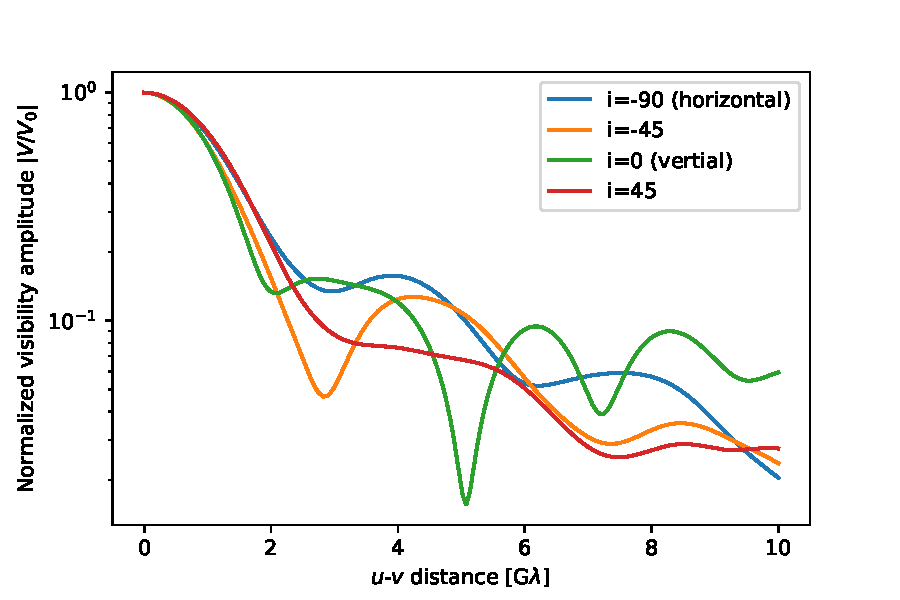
\includegraphics[width=0.5\textwidth]{figures/SANE_va.pdf}%
  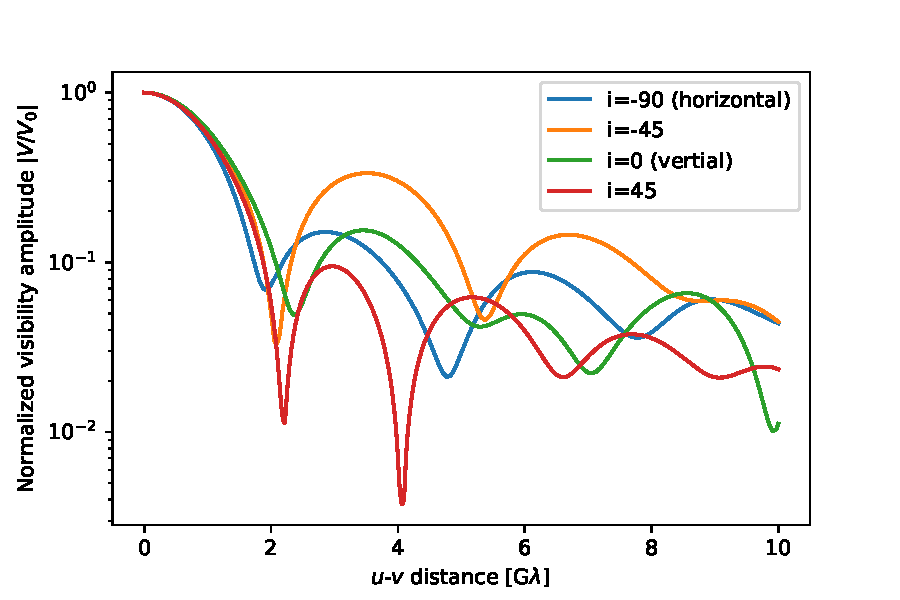
\includegraphics[width=0.5\textwidth]{figures/MAD_va.pdf}
  \caption{The left panels show two snapshots from a GRMHD simulation
    with SANE field configuration and black hole spin $a=0.5$ and the
    right panels the corresponding visibility amplitudes for a
    horizontal and a vertical cross section through the images.
    The snapshot in the top row obeys both selection criteria: the
    minima are in the 2.5-3.5 G$\lambda$ range and the amplitude in
    the $6-8$G$\lambda$ is below 6\%.
    The image in the bottom row, on the other hand, is an example that
    has no minimum in one cross section and too much power at long
    baselines, due to the asymmetry introduced by a transient bright
    structure in the flow.
    \ckc{The above plot looks odd because it's just one of the snapshot.  Do we want to show the mean?  The range?}}
  \label{fig:cmp_VA}
\end{figure*}

%\begin{figure}
%  \centering
%  \includegraphics[width=0.5\textwidth]{figures/va_compare.pdf}
%  \caption{Visibility amplitude as a function of baseline length
%    observed on 2017 April 7.
%    The pink band marks the location of the first minima in the
%    visibility amplitude along different orientations.
%    The horizontal red line marks our conservative upper limit for the
%    observed visibility amplitude between $6-8$G$\lambda$.}
%  \label{fig:cmp_null}
%\end{figure}

\begin{figure}
  \centering
  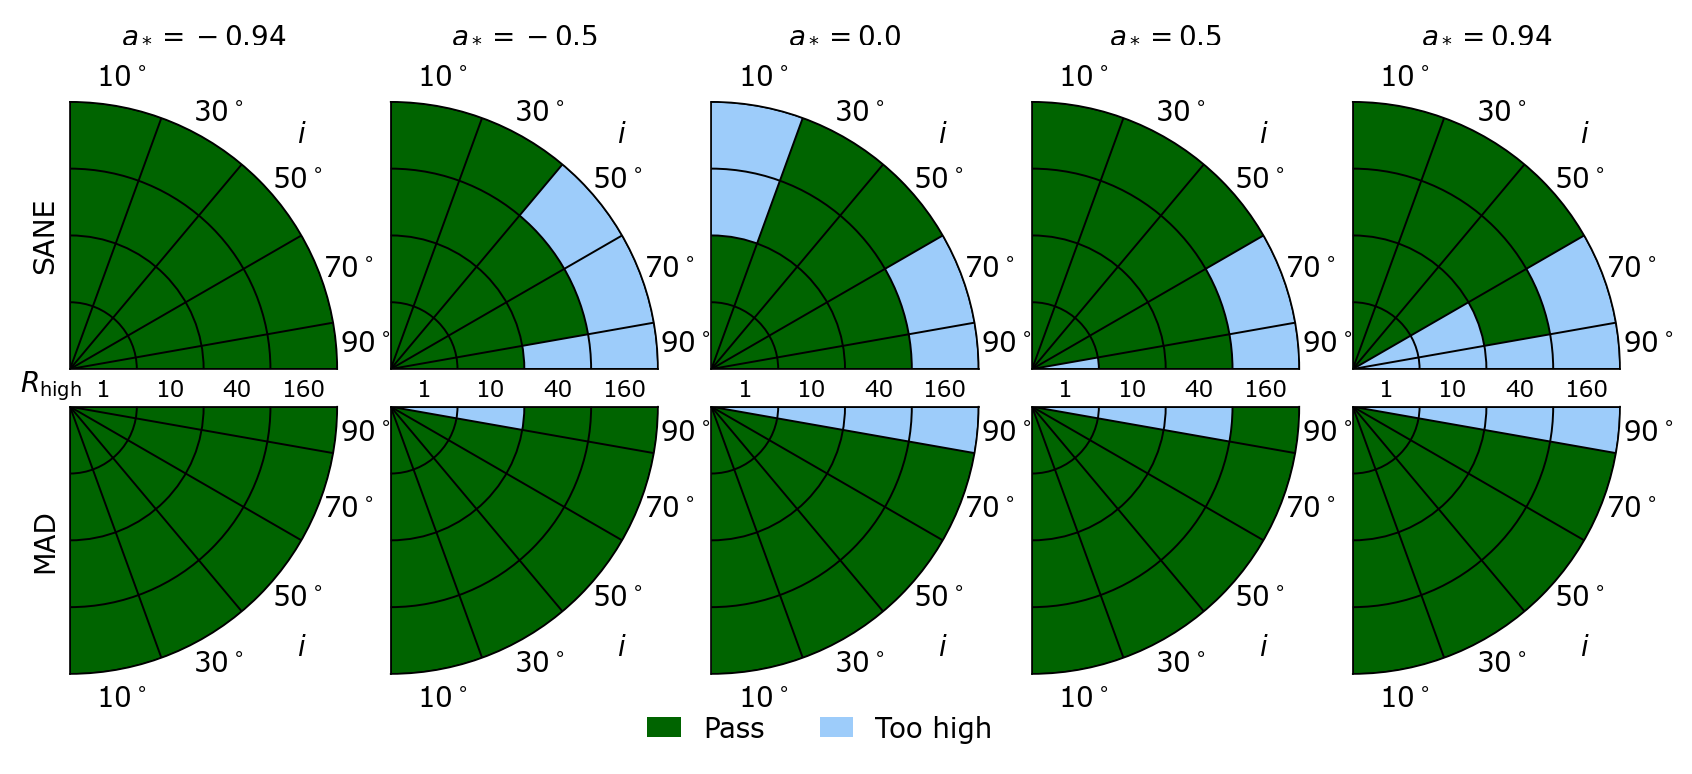
\includegraphics[width=\columnwidth]{./figures/Null_loc_Constraints.png}
  \caption{Null Location Constraint\ckc{Texts/labels in pizza plots too small to read.}}
  \label{fig:cmp_ozel}
\end{figure}

The null location constraint rules out edge-on MAD models at positive spin and a few large $\Rh$ SANE models.

The models that fail tend to...

Null location constraint passes 77\% of models.

%..............................................................................
\subsubsubsection{Second Moment}

\begin{figure}
  \centering
  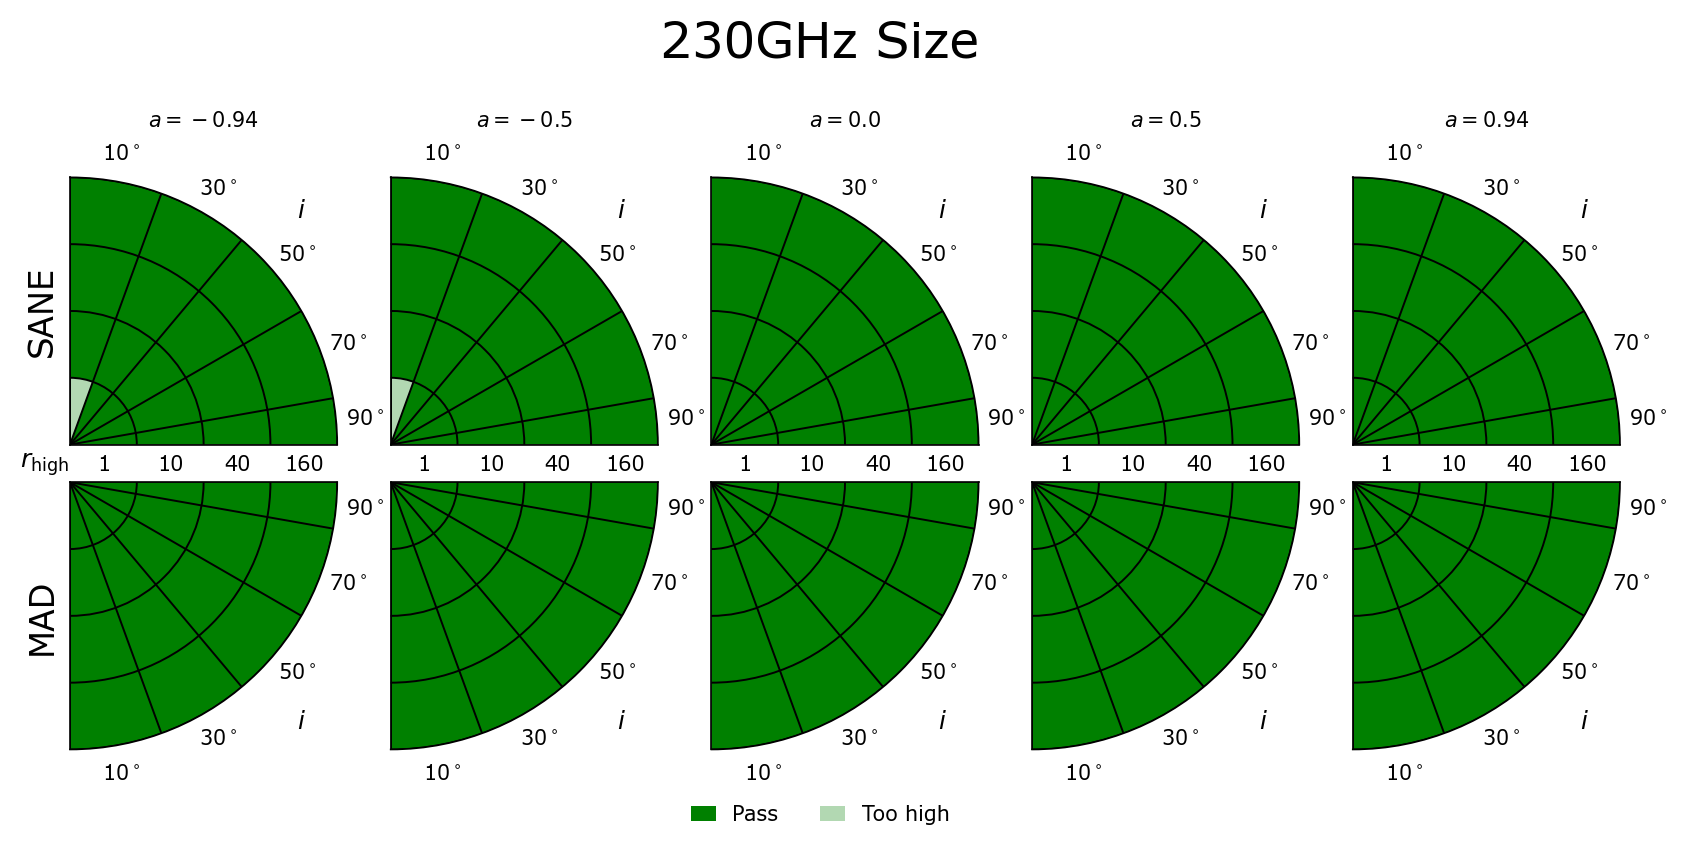
\includegraphics[width=\columnwidth]{./figures/230GHz_size_Constraints.png}
  \caption{2nd moment plots}
  \label{fig:cmp_2nd_moment}
\end{figure}

The second moment constraint passes 99\% of models, that is, the models are all crudely the right size.  The models that fail are retrograde, face-on, SANE models with $\Rh = 1$. These models have extended rings of emission with angular extent that is large compared to the critical impact parameter.

%..............................................................................
\subsubsubsection{M-ring Fits}
\label{sec:mring}

The m-ring fits pass 94\%, 65\%, and 36\% of models for the ring asymmetry, diameter, and width respectively.

The asymmetry parameter is typically not very well constrained.  The models that fail are almost all high inclination models with positive spin.  The failing models have asymmetries that are large and detectable because Doppler boosting concentrates emission in an equatorial spot on the approaching side of the disk.

\begin{figure}
  \centering
  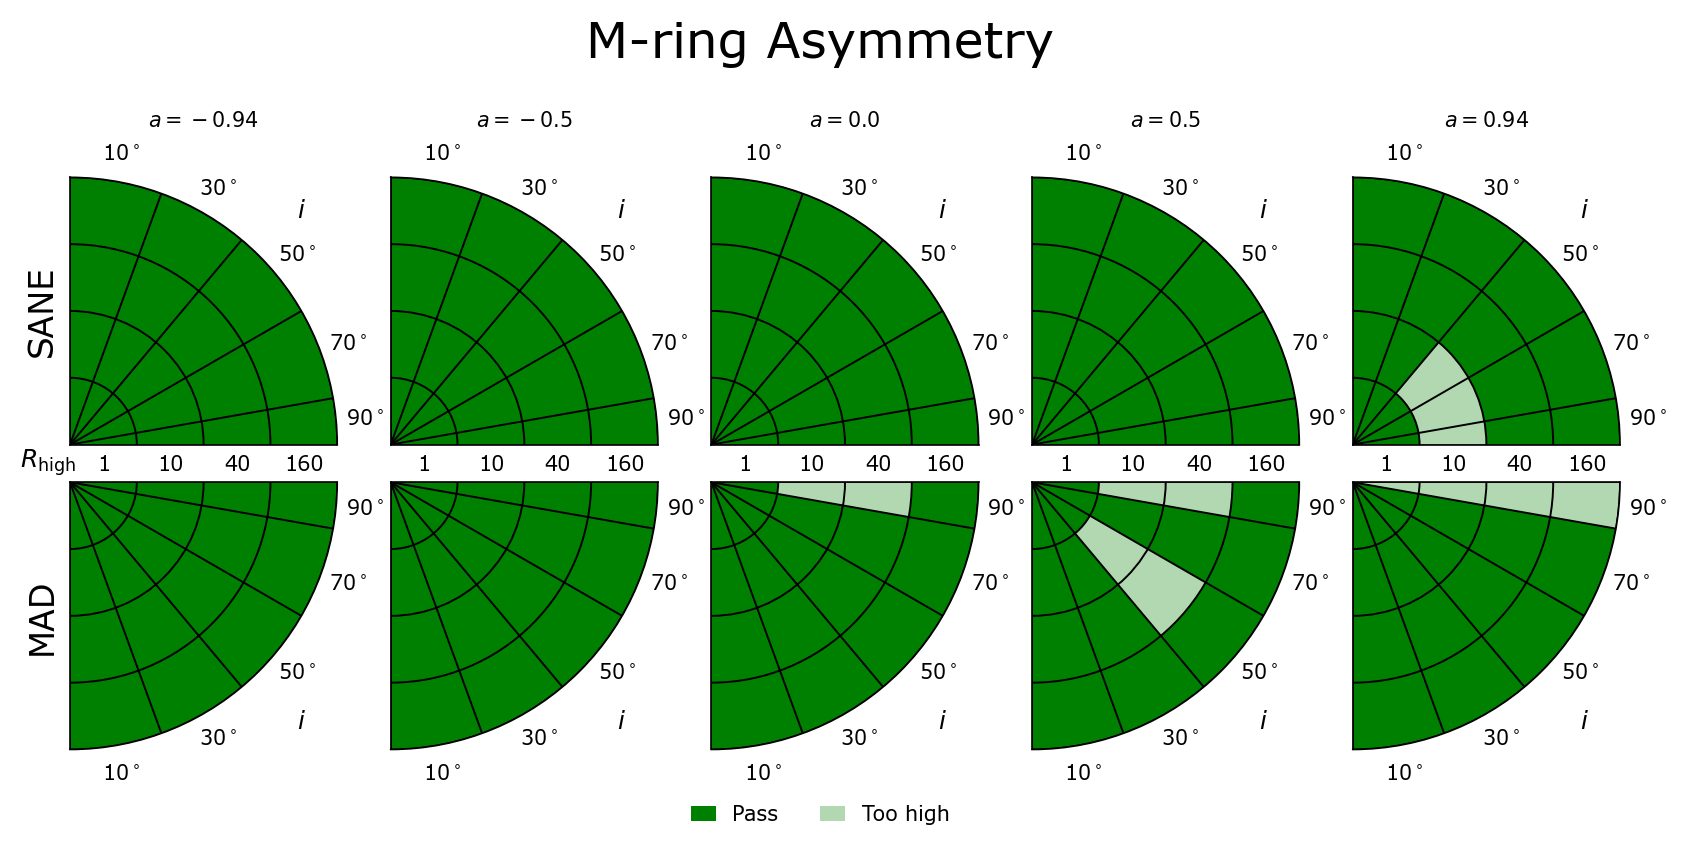
\includegraphics[width=\columnwidth]{./figures/Mring_f1_Constraints.png}
  \caption{m-ring asymmetry}
  \label{fig:cmp_m-ring_asymm}
\end{figure}

The ring diameter is better constrained than the asymmetry parameter.  It also varies systematically from model to model.  A much larger fraction of models therefore fails the ring diameter test.

Most of the models that fail are low inclination models with ring diameters that are too large (only one model fails because the ring diameter is too small).  For example, the face-on, $\Rh = 10$ SANE models fail for all spins except $\abh = 0.94$ because the ring is too large.  The same is true for all face-on MAD models with $\Rh = 1$.

\begin{figure}
  \centering
  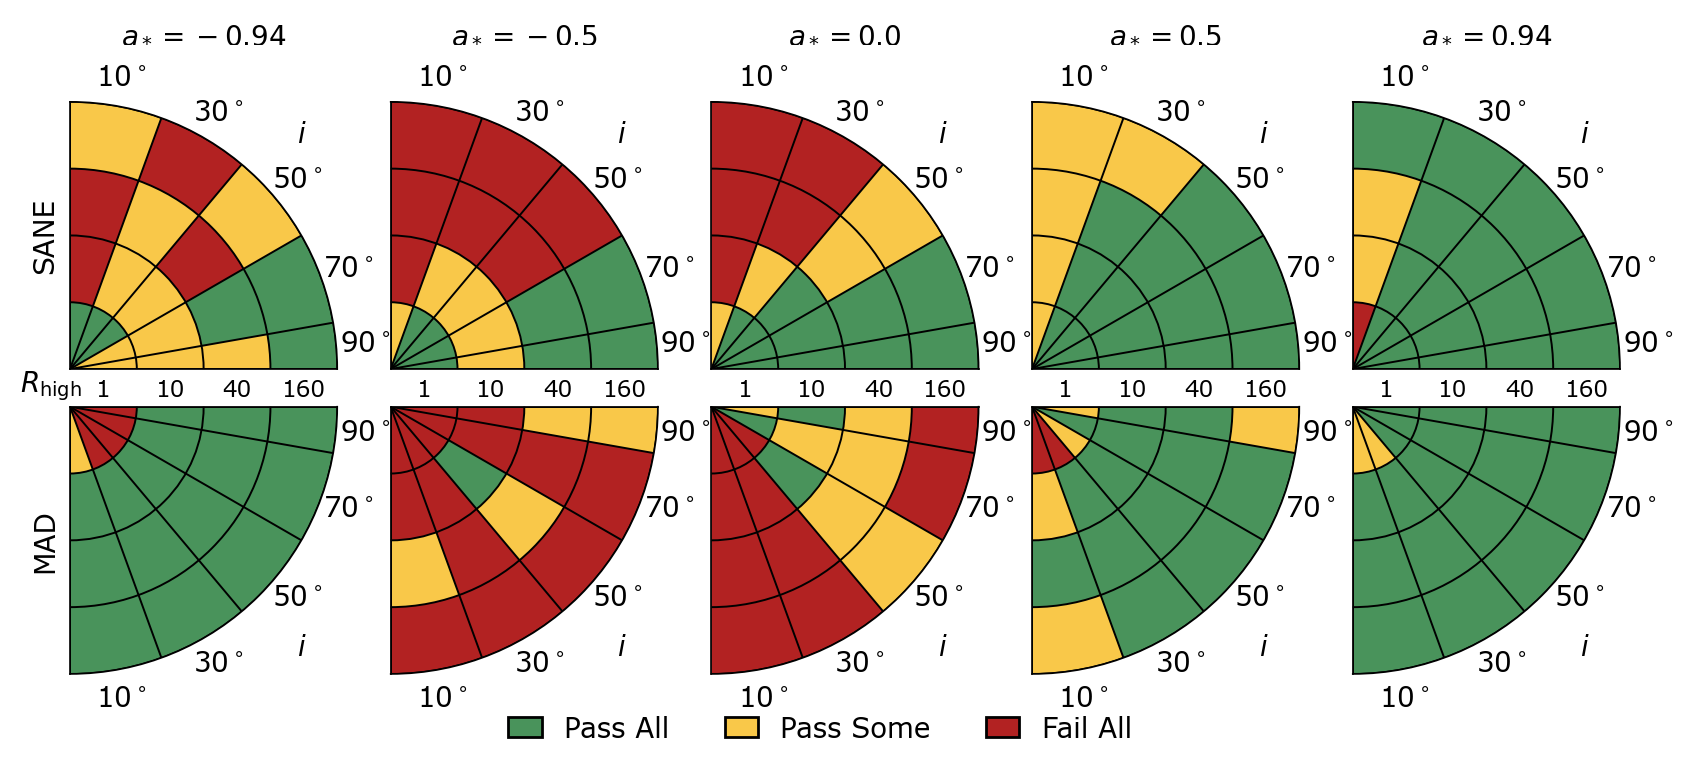
\includegraphics[width=\columnwidth]{./figures/Mring_d_Constraints.png}
  \caption{M-Ring diameter.}
  \label{fig:cmp_m-ring_diam}
\end{figure}

The m-ring width is best constrained and therefore most constraining.  Although the closure phases constrain the m-ring width as well, it is easy to see how the visibility amplitudes are affected by m-ring width: the width controls long-baseline amplitudes. Smaller width for a simple, symmetric ring corresponds to larger visibility amplitudes on long baselines.  

All models that fail have m-ring widths that are too small.  This includes all but 3 MAD models at $\abh \le 0$ and all MAD models at $i = 90\degree$.

\begin{figure}
  \centering
  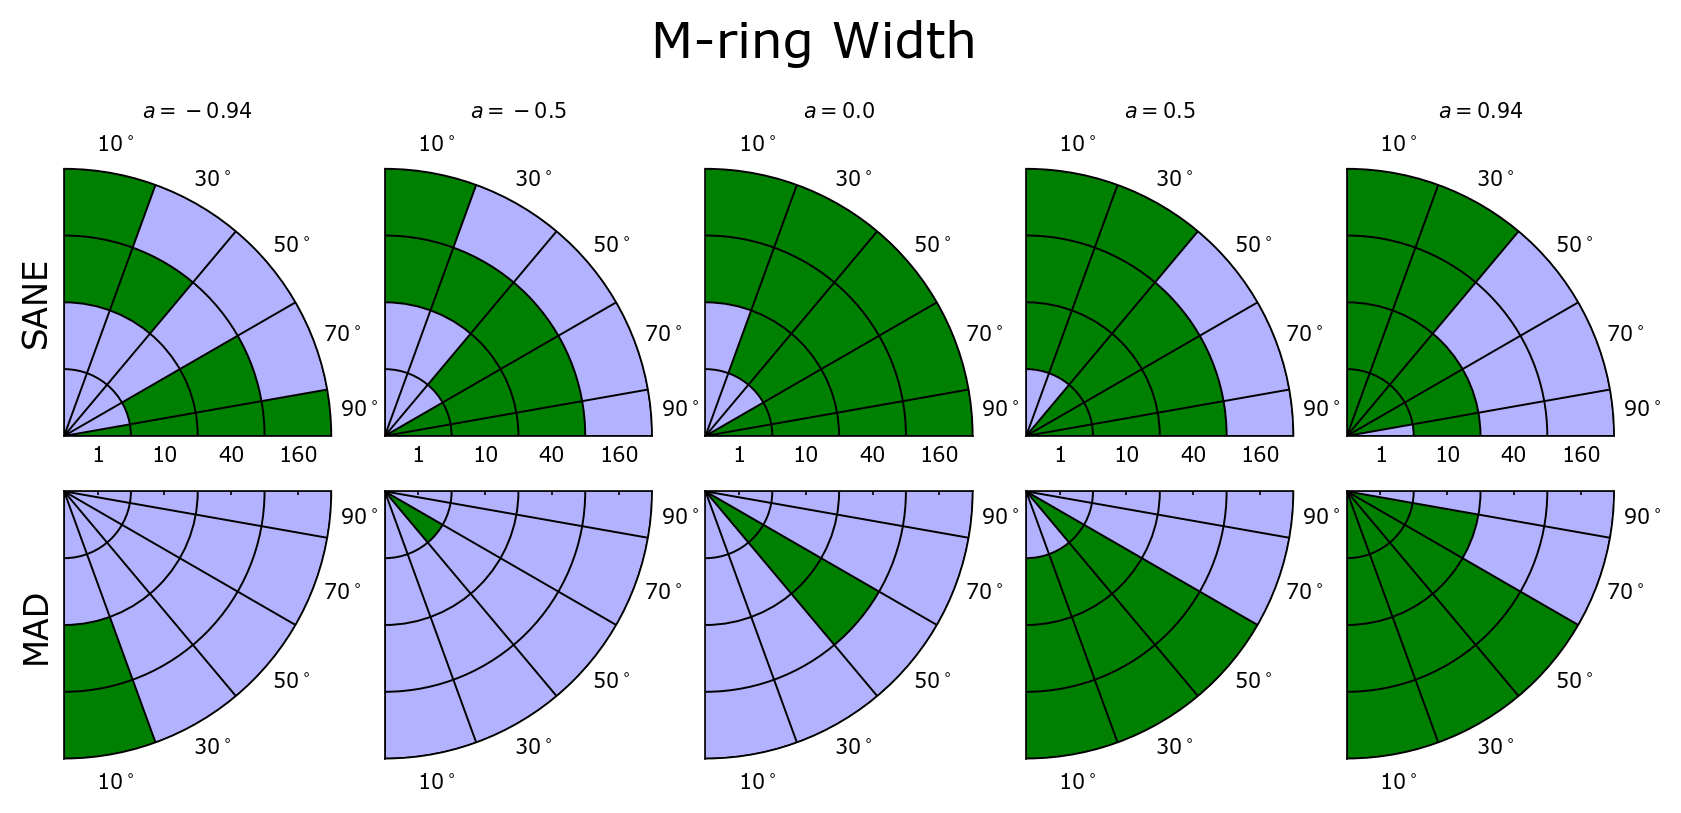
\includegraphics[width=\columnwidth]{./figures/Mring_w_Constraints.png}
  \caption{m-ring widths}
  \label{fig:cmp_m-ring_width}
\end{figure}

\subsubsubsection{EHT Constraint Summary}

Constraints based on EHT data are summarized in Figure \ref{fig:all_EHT_constraints}.  The cuts favor $\abh > 0$ models.  We are left with $31/100$ SANE models and $20/100$ MAD models.

\begin{figure}
  \centering
    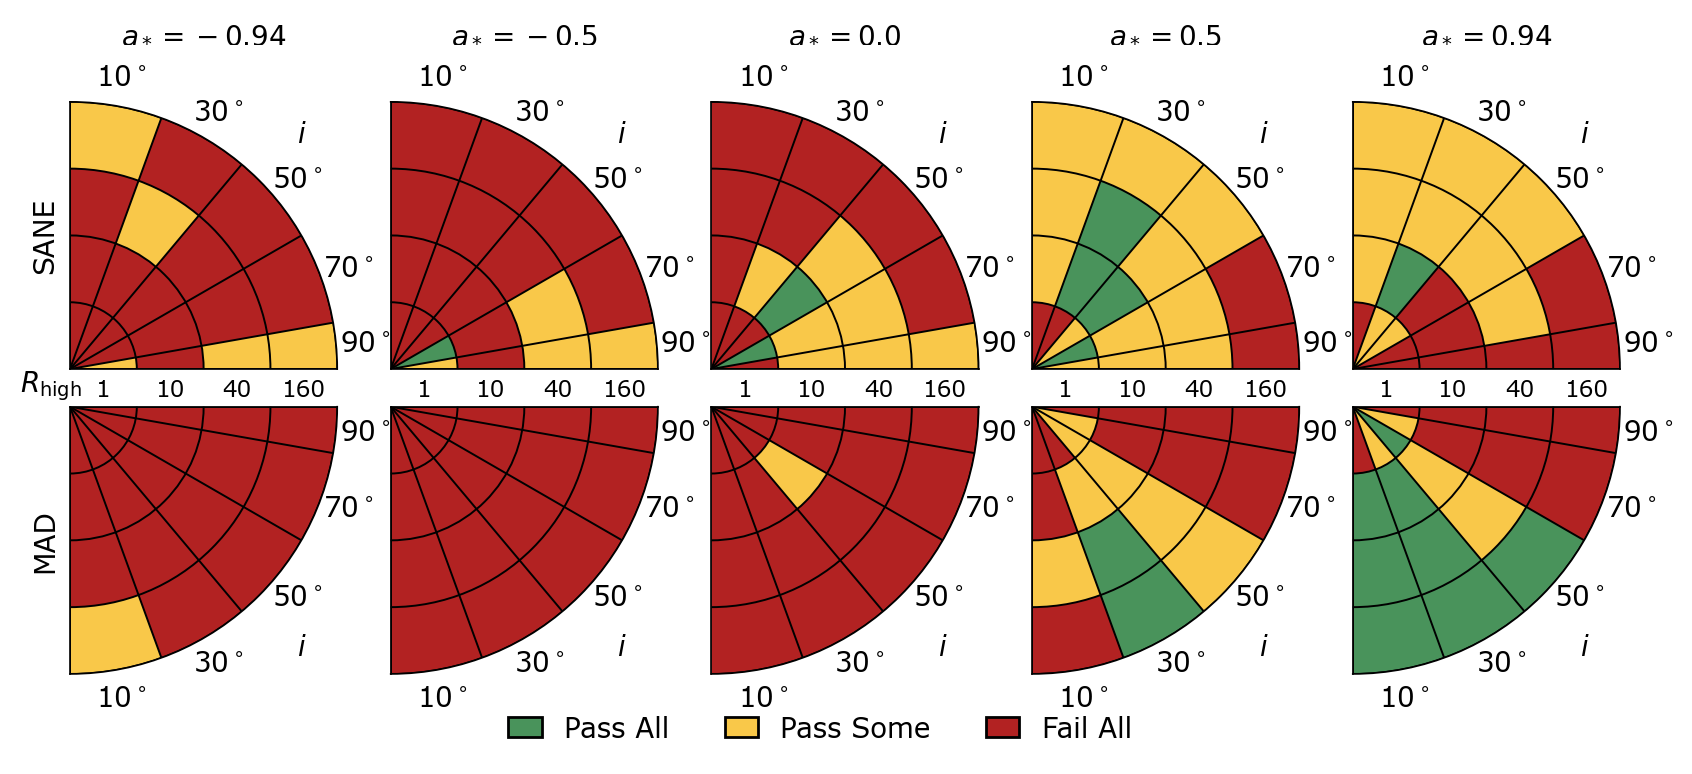
\includegraphics[width=\columnwidth]{./figures/Interferometric_Constraints.png}
  \caption{Combined EHT constraints (logical {\em and}) including the second moment, null location, and m-ring fit constraints.}
  \label{fig:all_EHT_constraints}
\end{figure}

\subsubsection{Non-EHT Constraints}

Now consider constraints from 86GHz, NIR, and X-ray observations.  Most or all of the emission in these bands is believed to originate in the compact source from plasma that is close to or overlaps the plasma the 230GHz-emitting plasma observed by EHT.

%..............................................................................
\subsubsubsection{NIR Median Flux}

\note{Michi}

NIR photons are produced by synchrotron process from photons at the high energy end of the distribution function.  For a one-zone model with $B = 30$G, the  critical frequency $\nu_{crit} \simeq \gamma^2 e B/(m_e c) \simeq 80$GHz and emission at $2.2\mu$m is therefore produced by electrons with $\gamma \simeq 10^3$, compared to a mean Lorentz factor of $30$ for plasma with $\Theta_e = 10$.  NIR flux density will therefore be sensitive to $\Theta_e$ and therefore to $\Rh$.

Interestingly, we find that some models are synchrotron-weak and Compton-strong in the NIR.  \note{Discussion of which models fall in this category}

Models that pass the NIR flux limit are shown in Figure \ref{fig:cmp_2um_flux}.

All but $6\%$ of the SANE models pass; the exceptions are high spin, high inclination models where Doppler boosting increases the NIR flux from the bright spot on the approaching side of the disk.

Considering MAD models alone, $68\%$ fail the NIR test, including all but 1 model at $\Rh = 1$ and $10$.

\begin{figure}
  \centering
  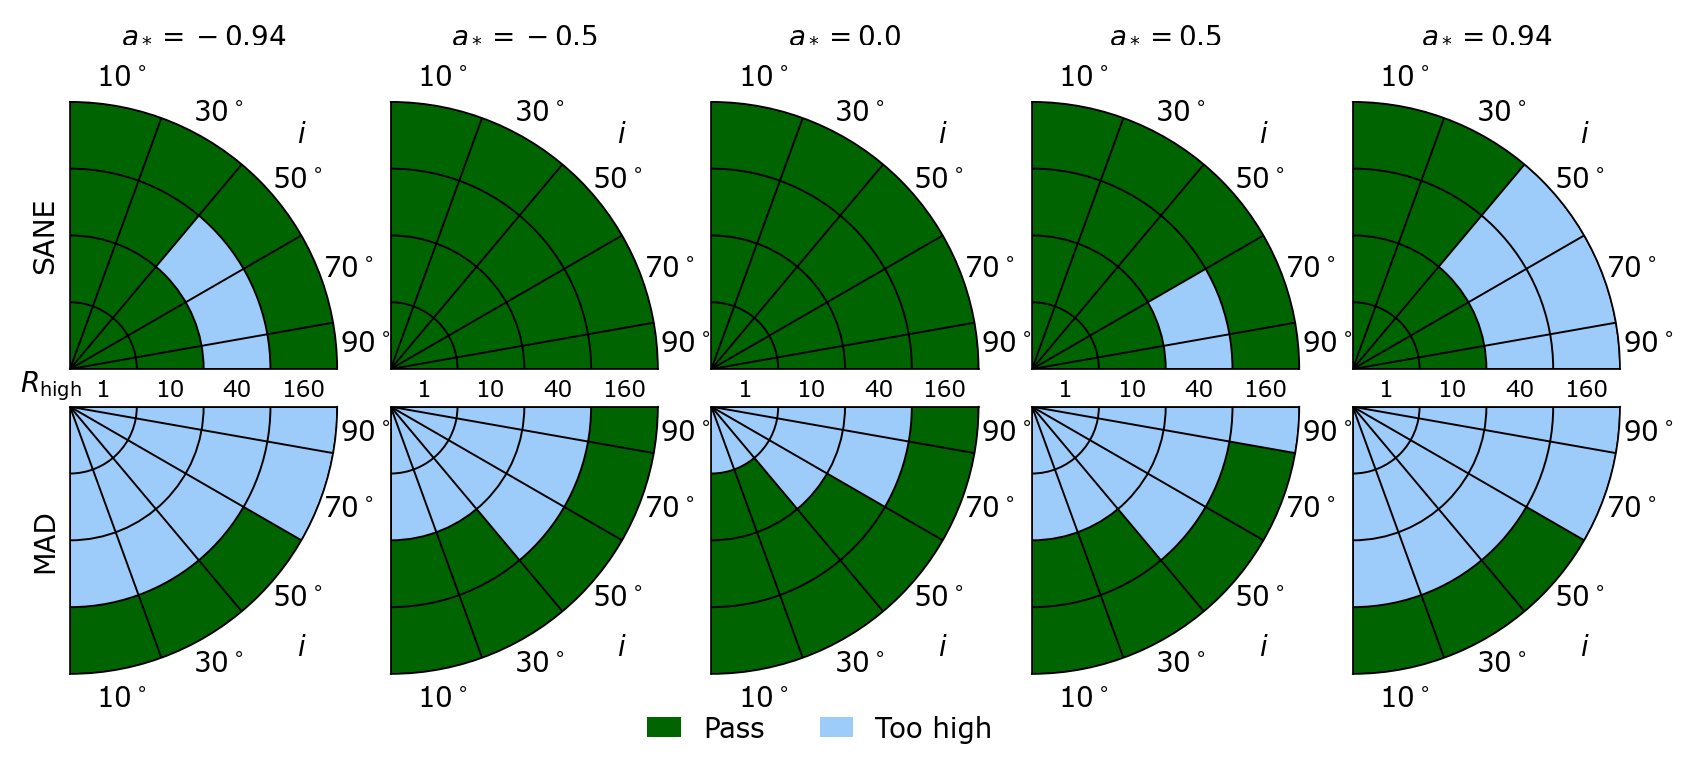
\includegraphics[width=\columnwidth]{./figures/2um_flux_Constraints.png}
  \caption{NIR flux limit}
  \label{fig:cmp_2um_flux}
\end{figure}

%..............................................................................
\subsubsubsection{X-ray Luminosity}

\note{Michi}

Most thermal models produce X-ray emission through Compton upscattering of thermal synchroton photons.  Typically the X-ray band lies in the first Compton bump, although that is sensitive to the temperature of the electrons doing the upscattering.  In the first Compton bump $\nu L_\nu$ is proportional to the y-parameter $y \sim 16 \Theta_e^2 \tau_e$ where $\tau_e$ is a characteristic electron-scattering optical depth and $\Theta_e$ is a typical electron temperature.

In many large $\Rh$ SANE models, however, X-ray emission is dominated by bremsstrahlung.  Since the bremsstrahlung emissivity $\propto n^2$, bremsstrahlung comes from the midplane where the density is largest, at larger radius than the synchrotron and Compton-upscattered X-ray emission.  It dominates in high accretion rate models (this turns out to mean large $\Rh$ models; see \S 5) where $\Theta_e < 1$, and is significant only when the midplane is cool and $r: \Theta_e = 1 < YY$, i.e. at large $\Rh$.  The resurgence of bremsstrahlung in cool disks occurs because at $\Theta_e < 1$, $j_\nu \propto n^2 \Theta_e^{-1/2}$.  When the disk is cool and dense the latter is large.

The e X-ray cut results are shown in Figure \ref{fig:cmp_xray_flux}.

Many large $\Rh$ SANE models fail the X-ray test: all but 3/25 at $\Rh = 160$ and all but 6/25 at $\Rh = 40$.  These models all fail due to excess bremsstrahlung.

Many MAD models that fail have large absolute spin and low $\Rh$.  These models are Compton-dominated.  The midplane temperature is highest at low $\Rh$.  Since the midplane contributes most of the electron scattering optical depth, low $\Rh$ models have the largest $y$ parameter and are therefore most at risk of overproducing X-rays.

\begin{figure}
  \centering
  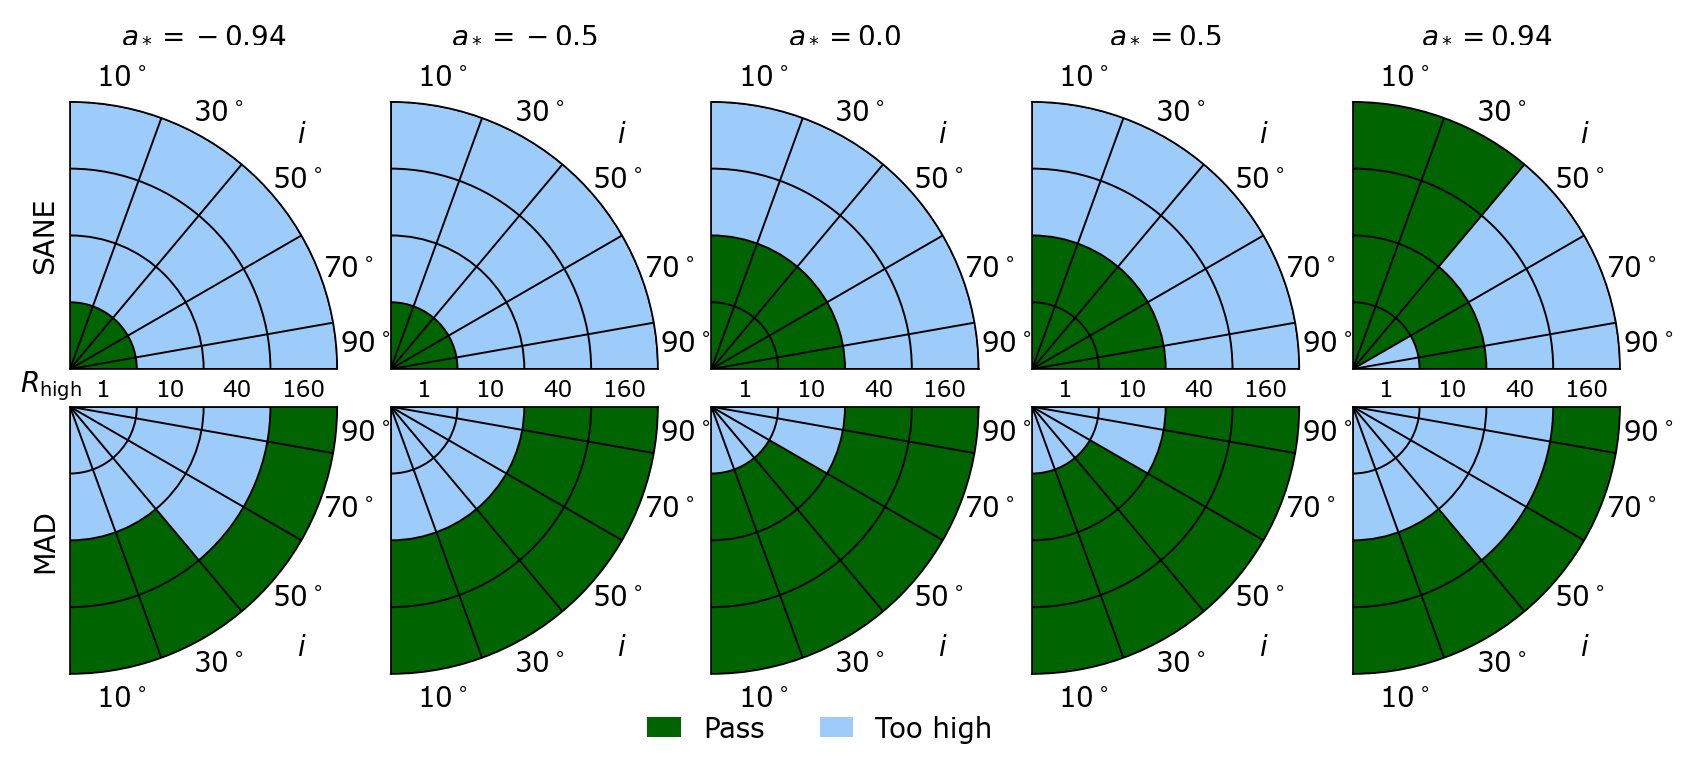
\includegraphics[width=\columnwidth]{./figures/Xray_flux_Constraints.png}
  \caption{X-ray flux limits}
  \label{fig:cmp_xray_flux}
\end{figure}

%..............................................................................
\subsubsubsection{86 GHz Median Flux}

In a naive picture \sgra's millimeter flux is produced at a photosphere that decreases in size as frequency increases.  Because of the marginal optical depth at $1.3$mm ($\sim 0.3$ in the one-zone model) and the complicated source structure (the optical depth varies across the image; the $\tau = 2/3$ surface is non-spherical, folded, and not even simply connected) this picture does not hold exactly.  Nevertheless 86GHz photons are typically produced at larger radius than 230GHz photons, and the 86GHz source size is therefore larger than the 230GHz source size; see Ricarte et al. 2021 for a discussion.

The 86GHz/230GHz color therefore probes the radial structure of the source plasma.  Figure \ref{fig:cmp_86ghz_flux} shows the result of requiring that the 86GHz flux match the observed flux 3 days before the beginning of the EHT 2017 campaign.

Many $\Rh = 1$ models, both MAD and SANE, fail the $86$GHz flux density test: 23/25 SANE and 9/25 MAD.  These models overproduce $86$GHz emission.
There are also a substantial set of SANE models, 19/100 in all, that underproduce $86$GHz emission.  These models have larger $\Rh$.

\begin{figure}
  \centering
  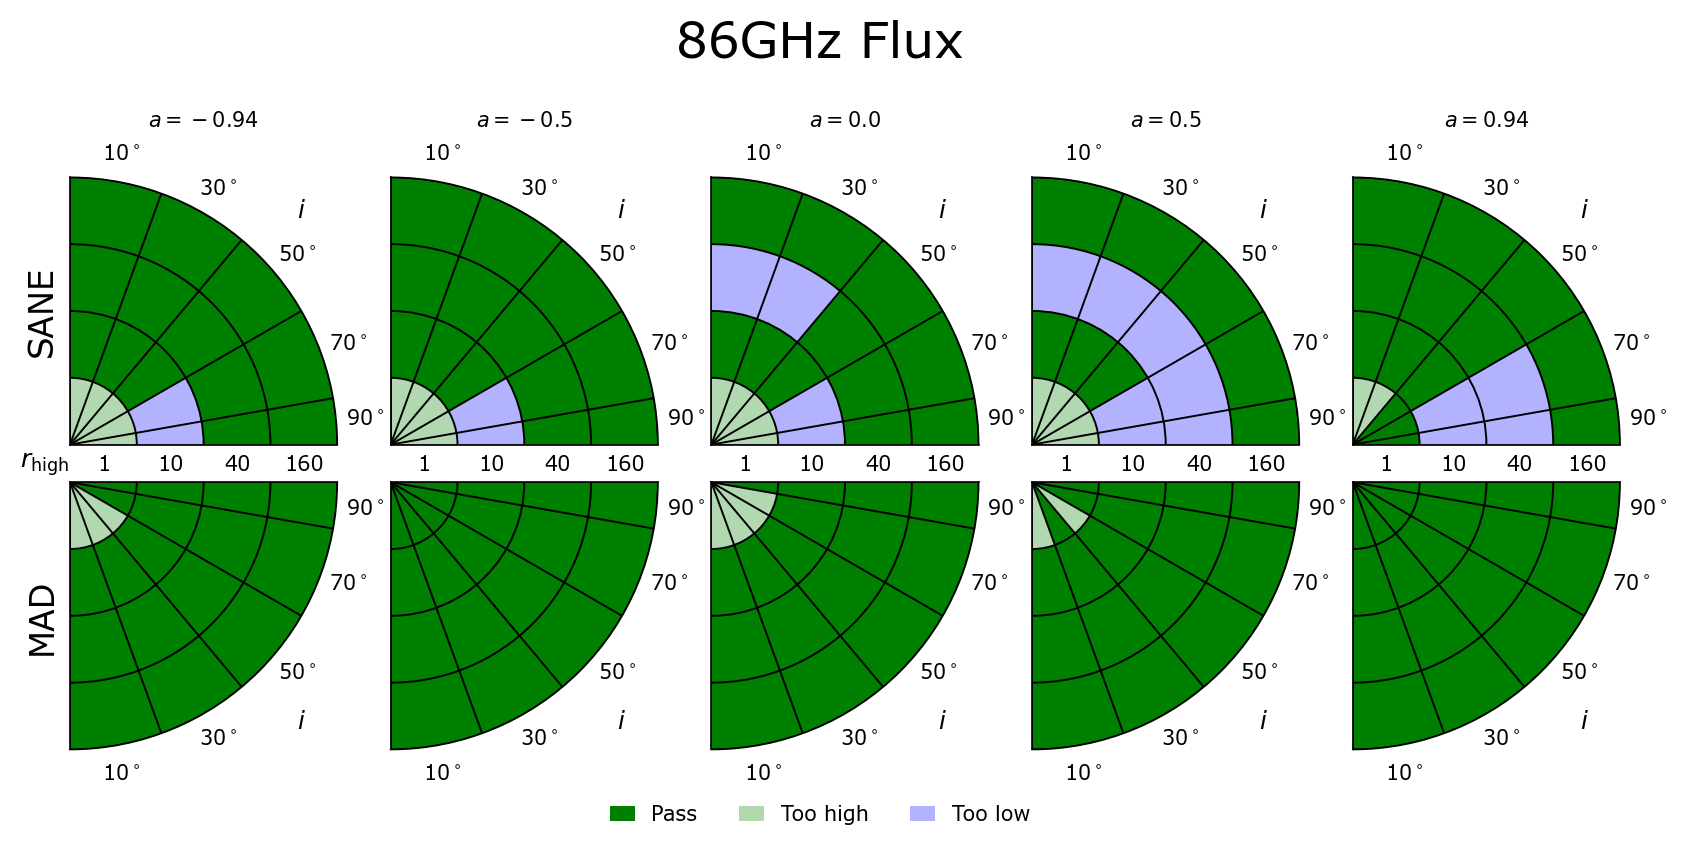
\includegraphics[width=\columnwidth]{./figures/86GHz_flux_Constraints.png}
  \caption{86GHz flux limits}
  \label{fig:cmp_86ghz_flux}
\end{figure}

\note{Michi}

%..............................................................................
\subsubsubsection{86 GHz Major Axis}

As for the $86$GHz flux, the $86$GHz size is sensitive to optical depth as a function of radius in the source plasma. Models that pass and fail are shown in Figure \ref{fig:cmp_86ghz_size}.

Many face-on models fail because they are too small (purple in the figure), while a few other high inclination models fail because they are too large.  Overall only about $50\%$ of models pass, making this one of the tightest constraints.

The physical picture for 86GHz source size is complicated, as is the extraction of the constraint itself from observations.  We note that (1) two different values for the 86GHz intrinsic source size have been reported in the literature; (2) scattering is $7$ times stronger at $86$GHz than at $230$GHz; (3) scattering must be subtracted accurately to obtain the intrinsic source size; (4) the error bars for the 86GHz source size are narrow and this determines the strength of the constraint.

\begin{figure}
  \centering
  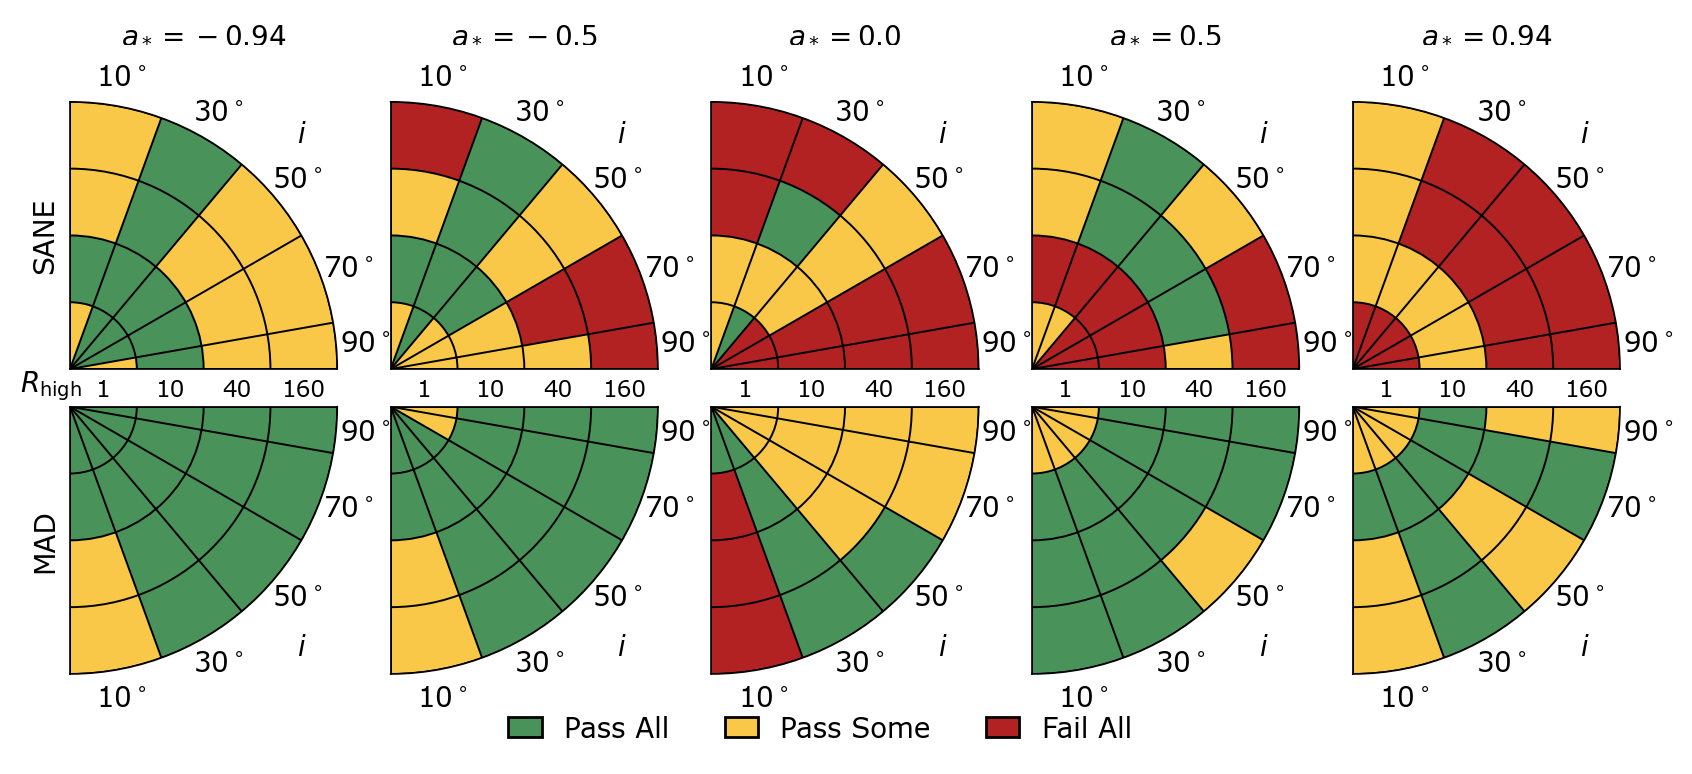
\includegraphics[width=\columnwidth]{./figures/86GHz_size_Constraints.png}
  \caption{86GHz size}
  \label{fig:cmp_86ghz_size}
\end{figure}

%..............................................................................
\subsubsubsection{Summary of Non-EHT constraints}

Applying only non-EHT constraints, we are left with the 9/100 SANE models and 25/100 MAD models shown in Figure \ref{fig:non_eht_cuts}.

The surviving models include a set of SANE models at intermediate $\Rh$ and modest inclination, as well as MAD models at large $\Rh \ge 40$.  No $\Rh = 1$ models survive the non-EHT cuts.

\begin{figure}
  \centering
  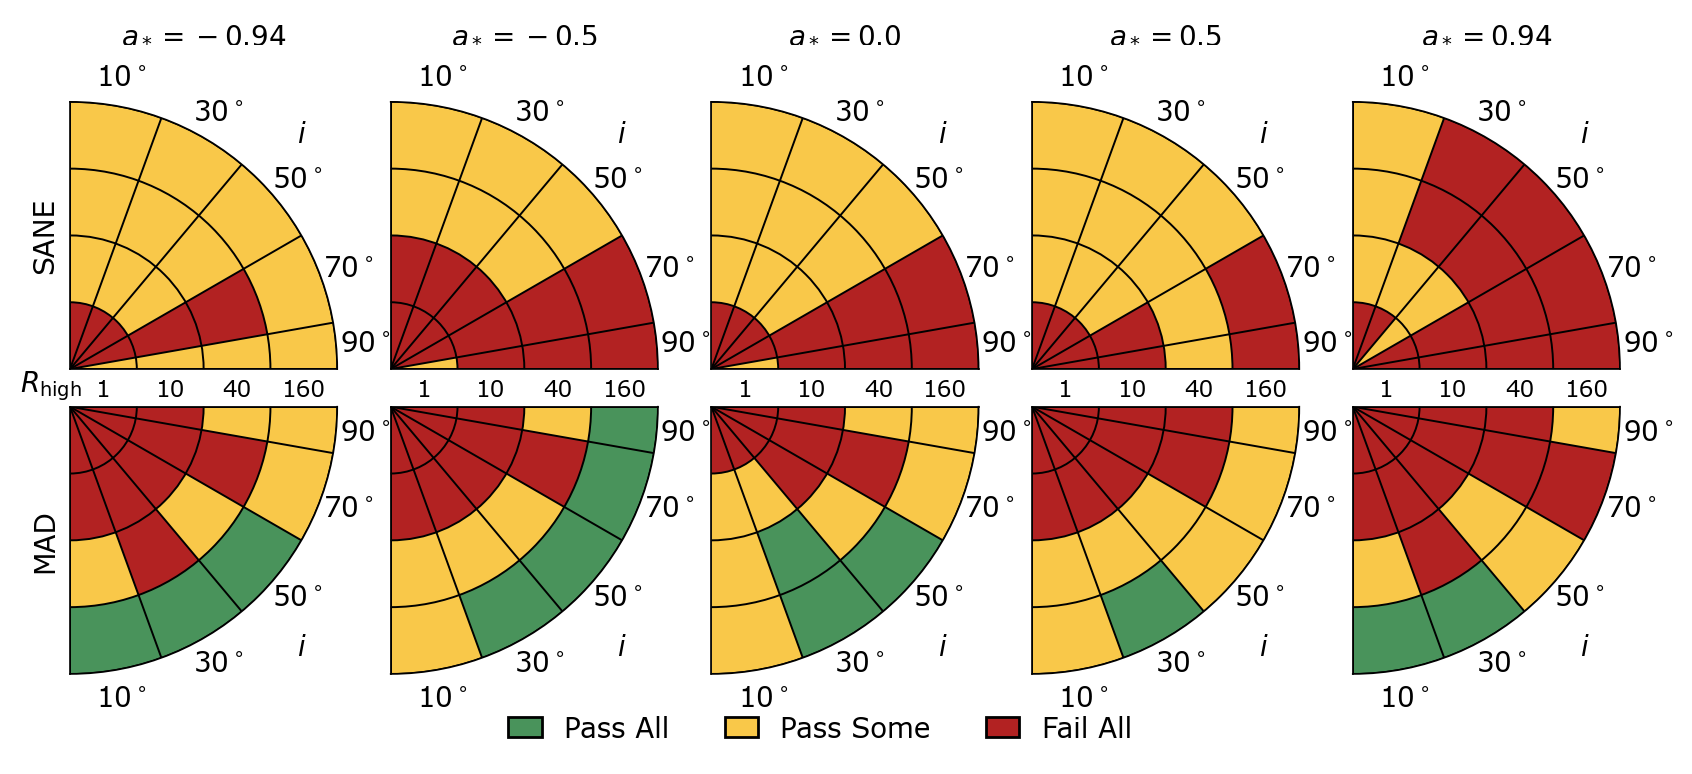
\includegraphics[width=\columnwidth]{./figures/Non_Interferometric_Constraints.png}
  \caption{Combined non-EHT constraints}
  \label{fig:non_eht_cuts}
\end{figure}

%------------------------------------------------------------------------------
\subsubsection{Variability}

Variability is central to interpretation of Sgr A*: the small black hole size means that observations considered here are taken over intervals when the source is expected to vary significantly.  This distinguishes Sgr A* from M87*, where the source is expected to vary only over timescales that are long compared to a single track.\footnote{Note, however, this does not suggest that M87* is less variable than \sgra.  Given the EHT only observed M87* at a few nearby snapshots, we cannot make any conclusive statement on M87* variability using EHT data alone.  To obtain the variability information we present here for M87*, it will require multi-year observations of M87*.}

Variability is a strong constraint on the models.  Although models differ in their degree of variability, both in an integrated sense and on 4 $G\lambda$ baselines, only a very small fraction of models are as quiet as the data.  For the light curve variability, this remains true whether we use data from 2017 April 7, all days from the 2017 observing campaign, or from historical monitoring of Sgr A*.   In general, SANE models are quieter than MAD models, and (less strongly) face-on models are quieter than edge-on models.

If we were to apply the variability constraints directly to the models, there would be 12/200 successful models left using 1\% cuts (65/200 for the ALMA constraint and 12/200 for the visibility amplitude constraint, with all models that pass the latter also passing the former)\dl{numbers and overlap between constraints subject to change}.  One interpretation of this result is that the surviving models are the correct description of the source (although we would expect some misclassification of models as consistent or inconsistent when using 1\% cuts on such a large model set).  Another interpretation is that there is a missing physical ingredient in the models, see Section \ref{sec:discussions} for a discussion.

%..............................................................................
\subsubsubsection{ALMA Light Curve}

The distributions of 3 hour modulation index (rms \%) across all SANE models, across all MAD models, and across the historical dataset are shown in Figure \ref{fig:cmp_ALMA_var}, along with individual distributions for the models with the lowest and highest MI for SANEs and MADs. Although individually, some models may pass (particularly SANE models), the distributions for the SANEs and the MADs are noticeably offset from the data, with the MADs in particular being more variable. As can be seen, even the quietest MAD model lies above the historical distribution. 

If we compare each individual model to the three segments from the 7 April 2017 ALMA observation using a 2-sample KS test, we find that 56 SANE models and 9 MAD models pass with $p > 1\%$. 

If we instead compare the models to the full historical distribution (40 3h MIs in all, including the ALMA MIs), we find that 53 SANE models and no MAD models pass with $p > 1\%$. This is more stringent than the comparison with just 7 April, since the historical distribution has more samples and thus disparate models can be eliminated with higher confidence. 

%If we compare each individual model to the five segments from the EHT 2017 campaign using a 2-sample KS test, we find that 80 (75) SANE and 21 (19) MAD models pass with $p > 1\%$. 

\begin{figure}
  \centering
  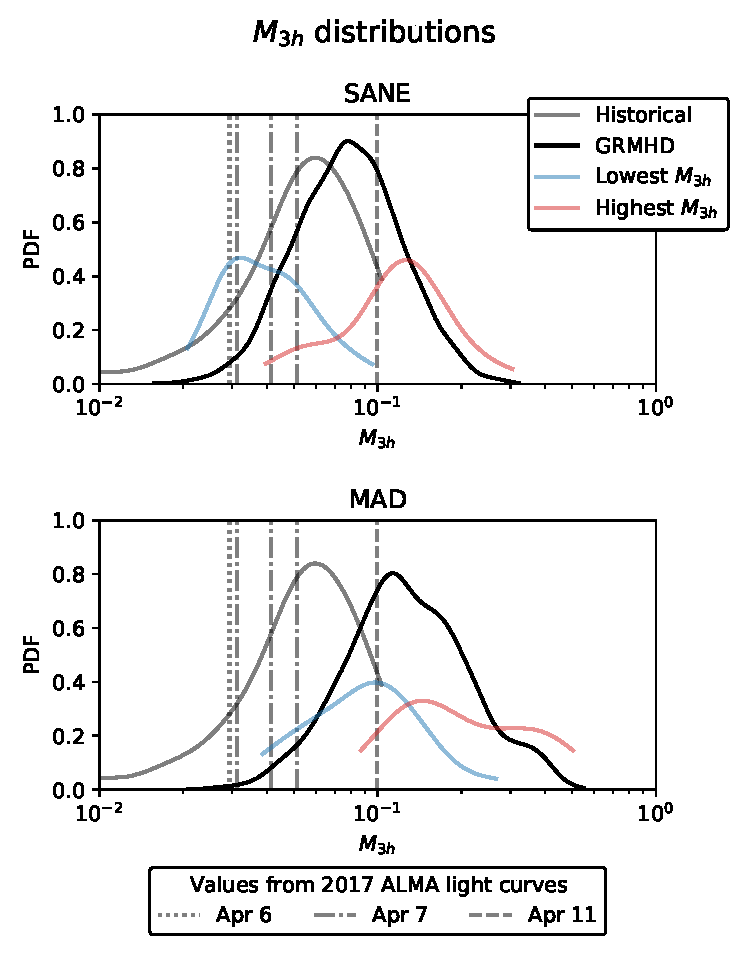
\includegraphics[width=\columnwidth]{./figures/mi_dist.pdf}
  \caption{Distributions of MI for Illinois thermal models (black), compared to distributions from historical observations (gray) and the values from the 2017 ALMA light curve. The latter are shown as vertical lines. The distributions for models with the lowest (blue) and highest (red) average MI for SANEs and MADs are also shown. }
  \label{fig:cmp_ALMA_var}
\end{figure}

%..............................................................................
\subsubsubsection{4 $G\lambda$ Visibility Amplitude Variability}

The distribution of model $4G\lambda$ lightcurve-normalized PSDs are shown in Figure \ref{fig:cmp_VLBI_var}.  The best fit PSD from the 2017 EHT campaign (excluding April 11) is shown as a solid vertical line, with the other vertical lines showing percentiles in the posterior.  Evidently the observations are quieter than both SANEs and MADs as a group.

The PSD estimates for the models are broken up into $5000\tg$ windows for each model. To compare the models to the observation, we take the mean value across all windows and assume the width of the distribution is of $\log_{10} a_{4G\lambda} \pm 0.1$. A model is considered passing if this estimated distribution overlaps with the median observed value. \note{refer GRMHD variability paper appendix} \dl{passing criterion subject to change}

With this approach only 6\% of the models pass, and all SANE. While the quietest models tend to be SANEs, the general distribution across all MADs is not as offset from the SANEs as in the MI distributions. 

\begin{figure}
  \centering
    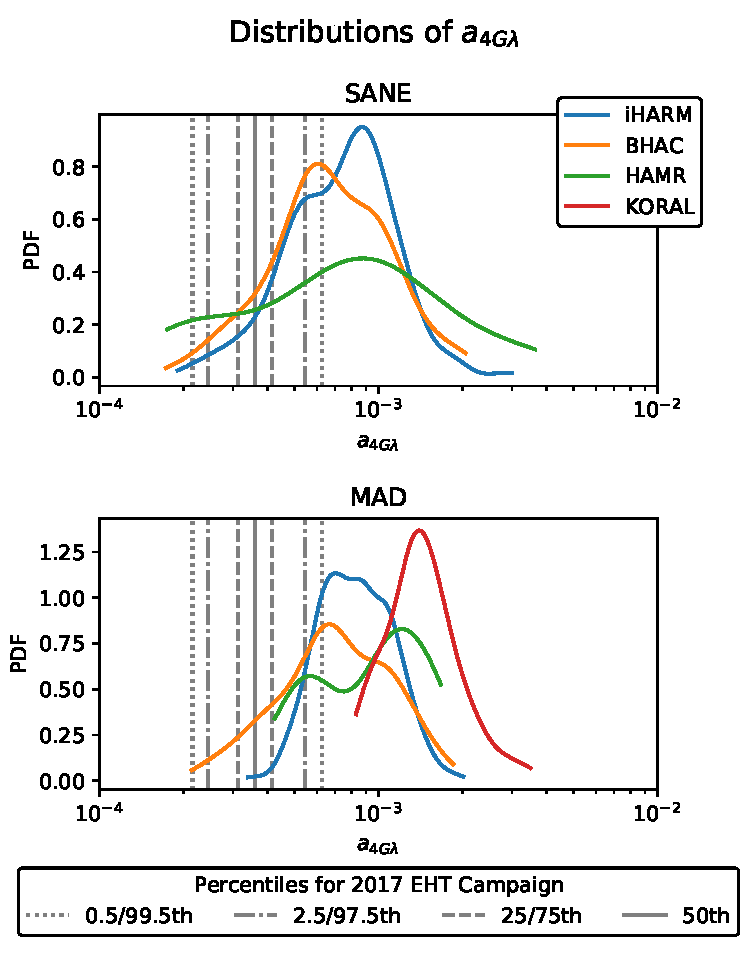
\includegraphics[width=\columnwidth]{./figures/va_dist.pdf}
  \caption{Distributions of $PSD(4G\lambda)$ for thermal models, compared to the observed distribution from the 2017 EHT campaign.
  \dl{HAMR distribution will be updated later. }}
  \label{fig:cmp_VLBI_var}
\end{figure}

At a 1\% cut, the models that pass the PSD constraint also all pass the MI constraint. It should be noted that this is partially because these constraints are weakly correlated \dl{also partially because we're imposing constraints differently between VLBI and light curve, and the light curve constraint is more lenient} None of the 12 models with acceptable variability pass the other tests.

%------------------------------------------------------------------------------

%------------------------------------------------------------------------------
\subsubsection{Summary of Constraints}

If we set aside variability constraints but use all the remaining constraints we are left with the models shown in Figure \ref{fig:all_cuts}.  Only 1/100 SANE models and 8/100 MAD models survive. The passing models cluster amongst low inclination ($i \le 50$deg) MAD models with $\Rh > 10$.

It is remarkable both that so many of the models look like the EHT data, lending confidence to the models, and that EHT data alone are capable of distinguishing between models in the model set, with only $N = 6$ antennas.  Future experiments with more antennas will contain much more information and provide even tighter constraints.

All $\Rh = 1$ models have been eliminated, most by multiple constraints, and we conclude that models with equal ion and electron temperatures are unacceptable.

All models with $i > 50$deg are eliminated, most by multiple constraints, and we conclude that high inclination models are disfavored.  In the SED edge-on models have a clear signature derived from Doppler boosting, with increased NIR and X-ray flux density.  In EHT constraints many edge-on models have a clear signature derived from low m-ring widths, strong asymmetry (although only for a few models), and failed null location constraint.

For thermal model sets both EHT and non-EHT constraints individually eliminate many models, but together the eliminate all but 5\%.  The success of the models for EHT constraints (apart from variability) supports the use of the models for applying non-EHT constraints and highlights the importance of contemporaneous monitoring of \sgra at other wavelengths.

\begin{figure}
  \centering
  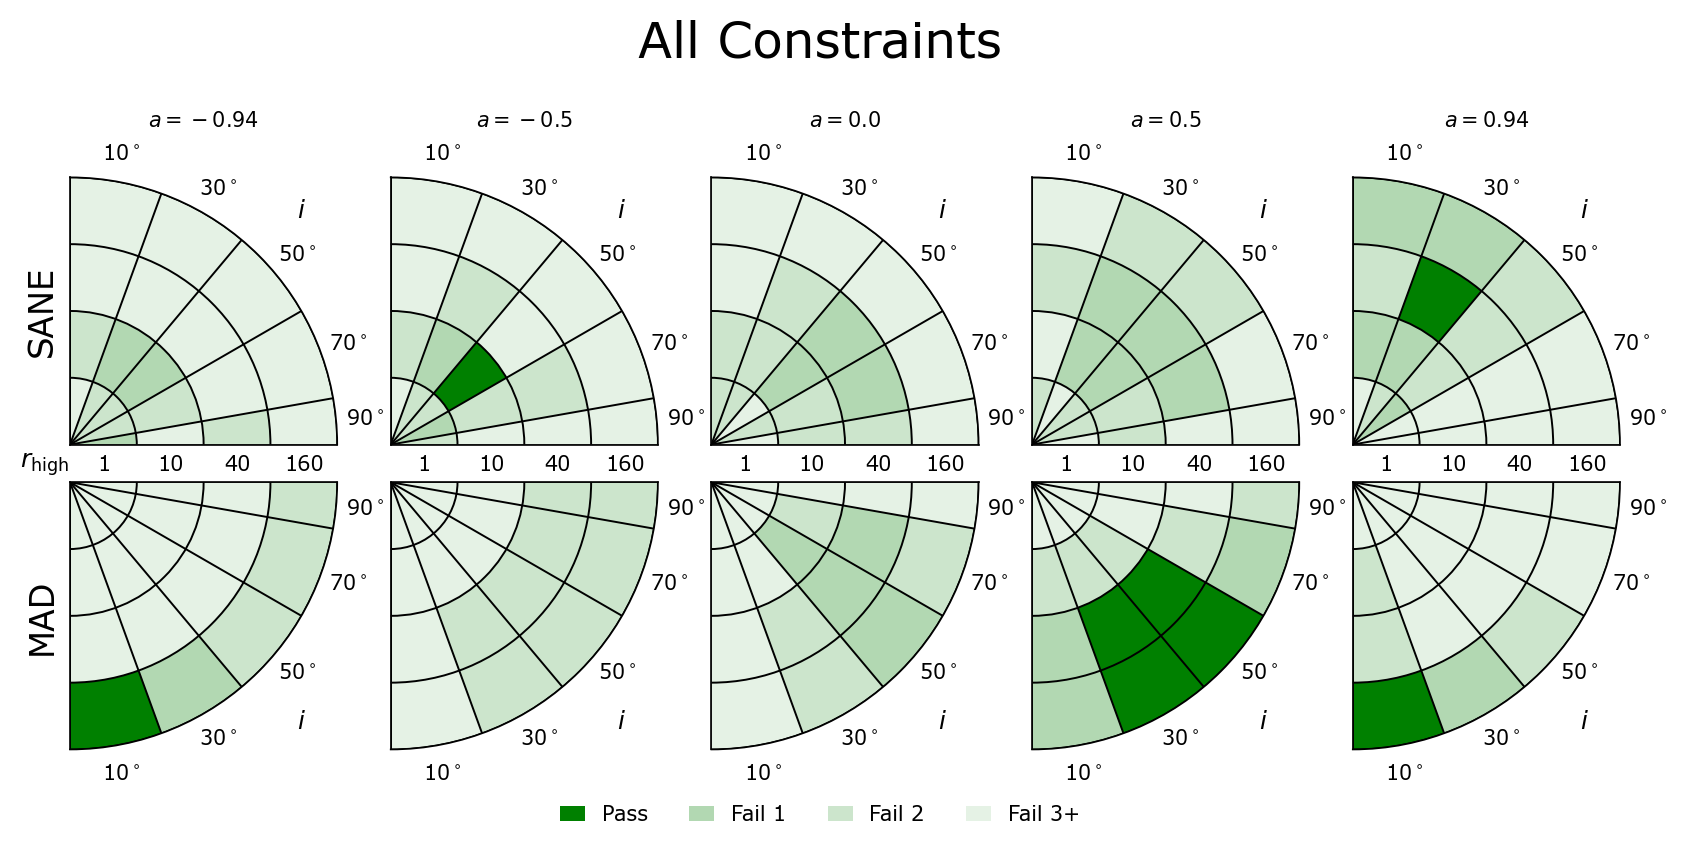
\includegraphics[width=\columnwidth]{./figures/All_Constraints.png}
  \caption{Combined EHT and non-EHT constraints}
  \label{fig:all_cuts}
\end{figure}

Variablity, were it included in the constraint map, would eliminate all thermal models.  Although a few models pass the variability constraints alone this does not mean that we should regard them as favored, since we are likely to find some false positives using a $1\%$ cut in a set of $200$ models.

%------------------------------------------------------------------------------
\subsubsection{Inter-Model Comparison for thermal models}

\cmf{First version}
As can be seen in Table \ref{tab:GRMHDmodels} the thermal models have been calculated for an identical parameter space from two different codes, namely iHARM and BHAC for the GRMHD simulations and iPOLE and BHOSS for the GRRT calculations. This allows us for the first time to perform an in depth comparison between the different numerical methods used in this work in addition to the EHTC code comparison projects \citep{2019ApJS..243...26P,2020ApJ...897..148G}.

\begin{figure}
  \centering
  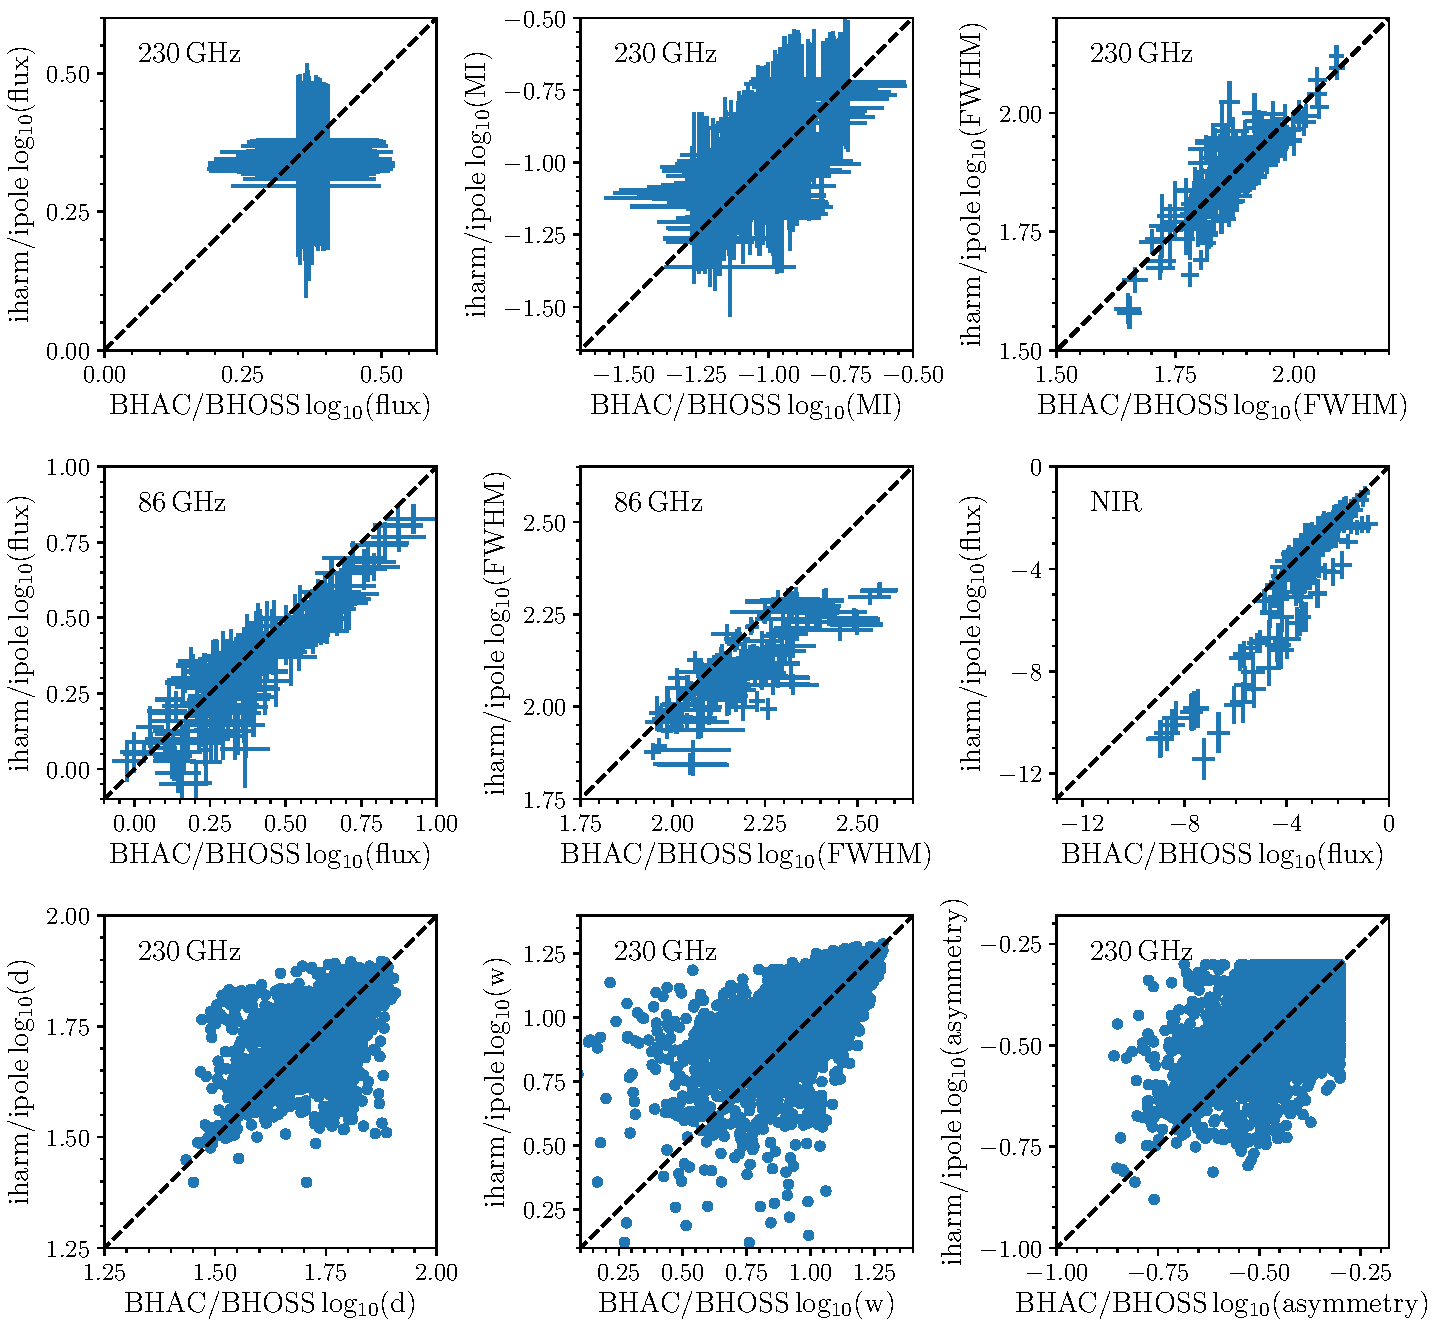
\includegraphics[width=\columnwidth]{./figures/BHAC_iharm_correlation}
  \caption{Correlation between BHAC and iHARM models based on model constraints}
  \label{fig:modelcorrelation}
\end{figure}

In Figure \ref{fig:modelcorrelation} we show the correlation between the thermal iHARM and BHAC models for various constraints.
\newline The top row shows from left to right the 230\,GHz flux density, the 230\,GHz modulation index, MI, computed for a time window of 3 hours, and the 230\,GHz image size obtained from image moments. Since we normalise the 230\,GHz images to an average flux of 2.4\,Jy within a time window of 5000\,M (corresponds to 28.5 h for SgrA a mass of $4.14\times 10^6\,\msun$), the scatter around this values is small. The deviation from an ideal correlation reflects the precision and number of GRMHD snapshots included during normalisation procedure.
\newline The correlation in the 3\,hour modulation index spreads over $\Delta \rm{MI}=0.75$ which reflects the intra-code ( e.g., MAD vs. SANE accretion and plasma models) and inter-code (BHAC vs. iHARM) differences. Despite these differences the models show a strong correlation throughout the investigated models and parameter space.
\newline We found a strong correlation between models and codes for the image size computed from image moments, i.e. second moments analysis. \\

The middle row presents the correlation plots for the 86\,GHz flux density (left), the 86\,GHz image size using second moments (middle) and the NIR flux (right). The 86\,GHz flux and 86\,GHz image size exhibit a shift toward larger values for the BHAC models. This difference can be explained by the larger field of view used for the BHAC models at 86\,GHz during the radiative transfer calculations. Thus, more extended structure and therefore a larger total flux is included in the BHAC models. This affects mainly models with large inclinations $i\geq70^\circ$ and jet dominated emission models ($\rm{R}_{\rm high}\geq 40$).
\newline The NIR fluxes show a tight correlation over four orders of magnitude and systematically larger flux for the BHAC models for low NIR fluxes ($\log_{10}(NIR)<-7$). These fluxes are far below the NIR constraints of $\sim 1mJy$, and therefore they do not affect the passing or failing of the models. In the thermal models the NIR flux is generated from the tail of the electron distribution function and thus very sensitive to the electron temperature. Thus, small differences in the distribution and value of the electron temperature between the two codes explain the observed de-correlation at very low NIR flux.  \\

The correlation between the models for the m-ring parameters is presented in the third row of Fig.~\ref{fig:modelcorrelation}. The correlation of the diameter of the m-ring is plotted in the left panel. The spread covers nearly the same extent as the 230\,GHz image size (top row, right panel) however the scatter in the correlation is larger.
The same is true for the width of the m-ring (middle panel in the last row of Fig.~\ref{fig:modelcorrelation}). Compared to the diameter and width of the m-ring, the asymmetry of the m-ring is less correlated (right panel). Notice, that the horizontal and vertical line in the asymmetries occurs since the parameter hits the boundary of the allowed range.

%\newline
The smaller correlation of the m-ring parameters as compared to the other parameters presented in Fig.~\ref{fig:modelcorrelation} can be
 understood by the different nature of the constraint i.e. image plane vs. Fourier space with sparse u-v coverage. For example, the m-ring fit fails for high inclination and large $\Rh$ values which leads to a large scatter in parameters for these models. %\\
%\newline
Nevertheless, the correlation between the two different codes and various models is astonishing and provides a robust basis for applied analysis and conclusions drawn from our model/image library.

%------------------------------------------------------------------------------
\subsubsection{Inter-Model Comparison}

\note{Doosoo, Koushik to write here about HAMR thermal models.  Define a subsection, describe the results.}

\note{Angelo and Richard to write here about critical beta models.  Define a subsection, describe the results.}

The $R$-$\beta$ model has been the default parametric model to span the vast uncertainties in emitting particle thermodynamics in EHT's computational pipelines. They are compatible with the well-motivated turbulent plasma heating ADAF models of \cite{1999ApJ...520..248Q} in asymptotic behavior of electron-to-total heating ratio as a function of plasma $\beta$. However, there is a vast function space of alternate interpolations with different behavior over various $\beta$ ranges.

The main theoretical motivation for the Critical Beta Model of \cite{2020MNRAS.493.1404A} is that when the transition between electron heating domination and proton heating domination is smoothed (controlled by increasing exponent parameter $\beta_c$), the 230 GHz emitting region profile tends to be less coronally dominated and more compact and asymmetric. This is a consequence, when fixing synthetic image flux, of higher critical beta values  shifting the locus of electrons dominating the emission profile towards a relativistically colder, higher density equatorial inflow.

Another motivation is that there are preliminary indications that the exponential electron cooling in the Critical Beta Model suppressed the SANE bremsstrahlung spectral component allowing more to pass the X-ray constraint.

%==============================================================================
\subsection{Nonthermal Aligned Models}

\note{Koushik to write here about powerlaw nonthermal HAMR models.  Define a subsection, describe the results and how they differ from the thermal results.][Maybe add Tomohisa's models here as well.] [by including power-law, we see this and that change (only include significant changes from the thermal models)}

\subsubsubsection{Constant power-law models $p=4.0$}




\note{Razi to write here about variable kappa models.  Define a subsection, describe the results and how they differ from the thermal results.}

\note{Christian to write here about constant kappa models.  Define a subsection, describe the results and how they differ from the thermal results.}\cmf{done}

%------------------------------------------------------------------------------
\subsubsection{Constant kappa models $\kappa=3.5$ with variable efficiency, $\varepsilon(\sigma,\beta)$}

In order to investigate the fraction on thermal to non-thermal particles we combine a thermal electron distribution function with a kappa electron distribution with $\kappa=3.5$. The value of $\kappa=3.5$ is motivated from the spectral slope in the NIR during a quiescent state \cmf{add reference here}. In addition to the fixed kappa value we assume that the fraction between thermal and non-thermal particles depends on the local plasma properties, e.g, the magnetisation, $\sigma$, and the plasma beta parameter, $\beta_{\rm p}$. Given this assumption we can write the total emissivity as:
\begin{equation}
j_{\nu,\rm{tot}}=\left[1-\epsilon(\varepsilon,\beta, \sigma)\right] j_{\nu,\rm{thermal}} + \epsilon(\varepsilon,\beta, \sigma) j_{\nu, \kappa},
\label{eq:kappaeff}
\end{equation}
where the efficiency, $\epsilon(\varepsilon,\beta,\sigma)$, is given by:
\begin{equation}
    \epsilon(\varepsilon,\beta,\sigma)=\varepsilon\bigg[1 - \exp\left(-\beta_{\rm p}^{-2}\right)\bigg]
    \left[1-\exp\left(\frac{-\sigma^2}{\sigma_{\rm min}^2}\right)\right].
    \label{eq:efficiencybetasigma}
\end{equation}
Throughout this work we fix $\sigma_{\rm min}=0.01$ and vary the base efficiency, $\varepsilon$, between 0.05, 0.1 and 0.2. For each base efficiency we generate a set of models spanning the same parameter space as the thermal models (see Table \ref{tab:radiativemodels} for details). For each model we iterate the mass accretion rate to obtain an average flux of 2.4\,Jy at 230\,GHz across a time interval of 5000\,M. In order to explore a several values of $\varepsilon$ we increased the cadence of the radiative transfer to 50\,M. This allows us to keep the numerical costs for this parameter sweep low while still being within the correlation time of the GRMHD simulations ($t_{\rm corr}\approx 50-100\,M$) \cmf{ do we have reference for this? So far this result is not published, maybe Boris paper?}. An example for the distribution of the efficiency can be seen in the right half of  Fig. \ref{fig:varepsilon}. The efficiency quickly approaches $\epsilon=0$ within the disk region while within the jet the efficiency reaches the defined base-efficiency. Thus, togehter with the used cut of in sigma, $\sigma_{\rm cut}=1$ the non-thermal particles are mainly located in jet sheath.

\begin{figure}
  \centering
    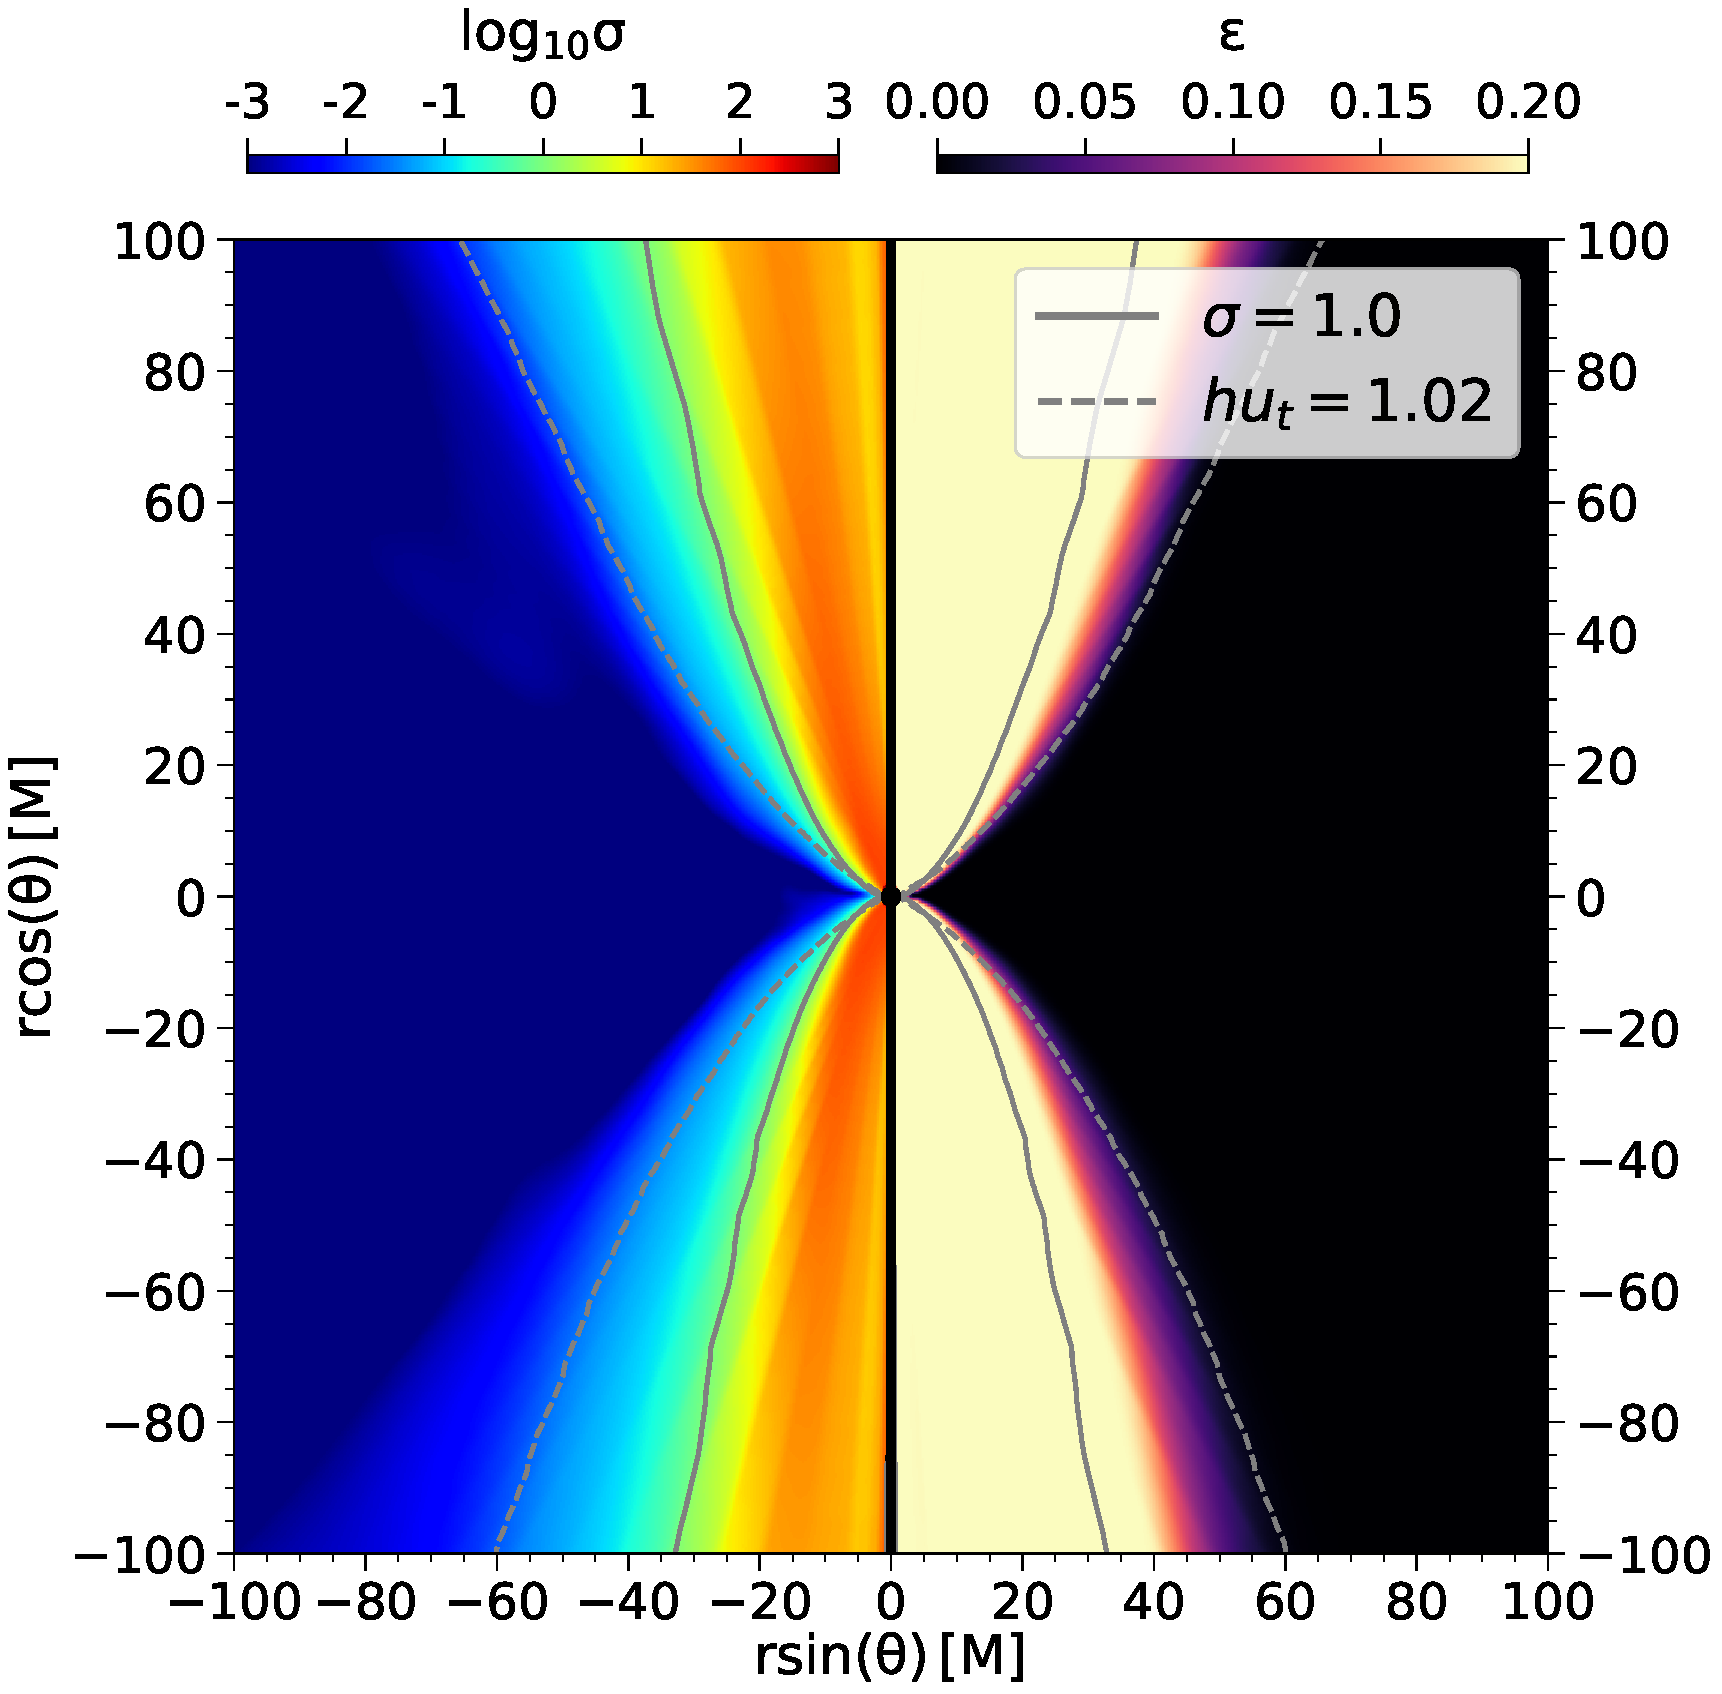
\includegraphics[width=\columnwidth]{./figures/GRMHDphiavera0.94sigmaeta.pdf}
  \caption{Time and azimuthal averaged distribution of the magnetization, $\sigma$ (left half) and the efficiency, $\epsilon(\varepsilon,\beta,\sigma)$ using $\varepsilon=0.2 $ for a BHAC MAD GRMHD simulation with spin $a_{\star}=0.94$. The solid gray line corresponds to $\sigma=1$ and the dashed line indicates out-flowing plasma via the Bernoulli parameter ($-h u_{t}>1.02$).}
  \label{fig:varepsilon}
\end{figure}

In the following we will elaborate the impact of adding non-thermal particles via the kappa electron distribution with fixed kappa value ($\kappa=3.5$) and there different base efficiencies $\varepsilon=$0.05, 0.1 and 0.2 on the observational constraints listed in Sect. \ref{}.

%..............................................................................
\subsubsubsection{230\,GHz VLBI pre-image size}

The addition of non-thermal particles alters the 230\,GHz VLBI pre-image sizes hardly for the MAD models and shows a minor effect on the SANE models. In the SANE case only models with $\Rh>40$ exhibit a minor increase in the source size where we see a monotonic increase of the source size with inclination. This effect can be understood if we consider that the bulk of the emission in all cases consider here is still produce by the thermal electron distribution, their temperature is given by Eq. \ref{} and an increase in $\Rh$ suppresses the emission from particles in the disk (by decreasing the electron temperature) and thus enhances the emission from jet.
Given that most the non-thermal particles are located in the sheath of the jet their impact on the source size is largest if bulk of the thermal emission is also produced there. In addition the emissivity of thermal synchrotron radiation decreases as $j_{\nu}\propto \exp{\left(-\nu^{1/3}
\right)}$ while for the kappa distribution as $j_{\nu}\propto \nu^{-(\kappa -2)/2}$. This implies that for the same electron temperature the non-thermal flux is compared to a thermal one higher and thus leads to a more extended jet structure for the models including non-thermal particles.
\newline In the MAD case, independent of the choice of $\Rh$ the emission is mostly produced in the disk region (see EHT paper V and Fig 8 in Wong et al. 2021 for 3D rendering). Increasing $\Rh$ will not push the emission region into the jet where the non-thermal particles are located and thus their contribution to the total emission structure is negligible.

%..............................................................................
\subsubsubsection{86\,GHz flux}

Since the GMVA+ALMA observations at 86\,GHz \cmf{ref to Issaoun paper} probe a larger field of view as the 230\,GHz EHT observations, we increased the field of view for the 86\,GHz to 800\,$\rm{\mu as}$ during the radiative transfer calculations. As mentioned earlier the non-thermal particles are mainly located in the jet sheath and thus the increased field of view ensures that no extend flux is missing during the comparison with the 86\,GHz observations.
\newline The 86\,GHz for both SANE and MAD models flux is not affected by the addition of non-thermal particles. In case of the SANE models the edges of the 86\,GHz flux distribution are slightly shifted in the case of $\Rh>40$. However, including non-thermal particles even with the highest base efficiency $\varepsilon=0.2$ does not change the scoring of a model, i.e., a thermal-only model which full-fills the 86\,GHz constrain is still accepted if non-thermal particles are included. This behaviour can be explained by the fact that the bulk of the emission in both accretion models is generated in with a few gravitational radii. Since the non-thermal particles are mainly located in the jet sheath and thei ratio between non-thermal to thermal particles is at most 20\% the contribution of the non-thermal particles to the 86\,GHz flux can be neglected.

%..............................................................................
\subsubsubsection{86\,GHz image size}

The behaviour of the 86\,GHz image size is very similar to the above described 230\,GHz image size: There is no change in image size for the MAD models and only a minor increase in the SANE models for $\Rh>40$. The physical reasons for this behaviour follows the same arguments as in the 230\,GHz VLBI pre-image size.

%..............................................................................
\subsubsubsection{NIR constraints}
As expected, the addition of non-thermal particles via the kappa electron distribution function with variable efficiency has a large influence on the NIR flux for all models independent of the accretion model and the $\Rh$ value. In Fig.~\ref{fig:NIR_kappaepsilon} we compare the distribution of the NIR fluxes for thermal and kappa eDF for a SANE accretion model.

\begin{figure}
  \centering
  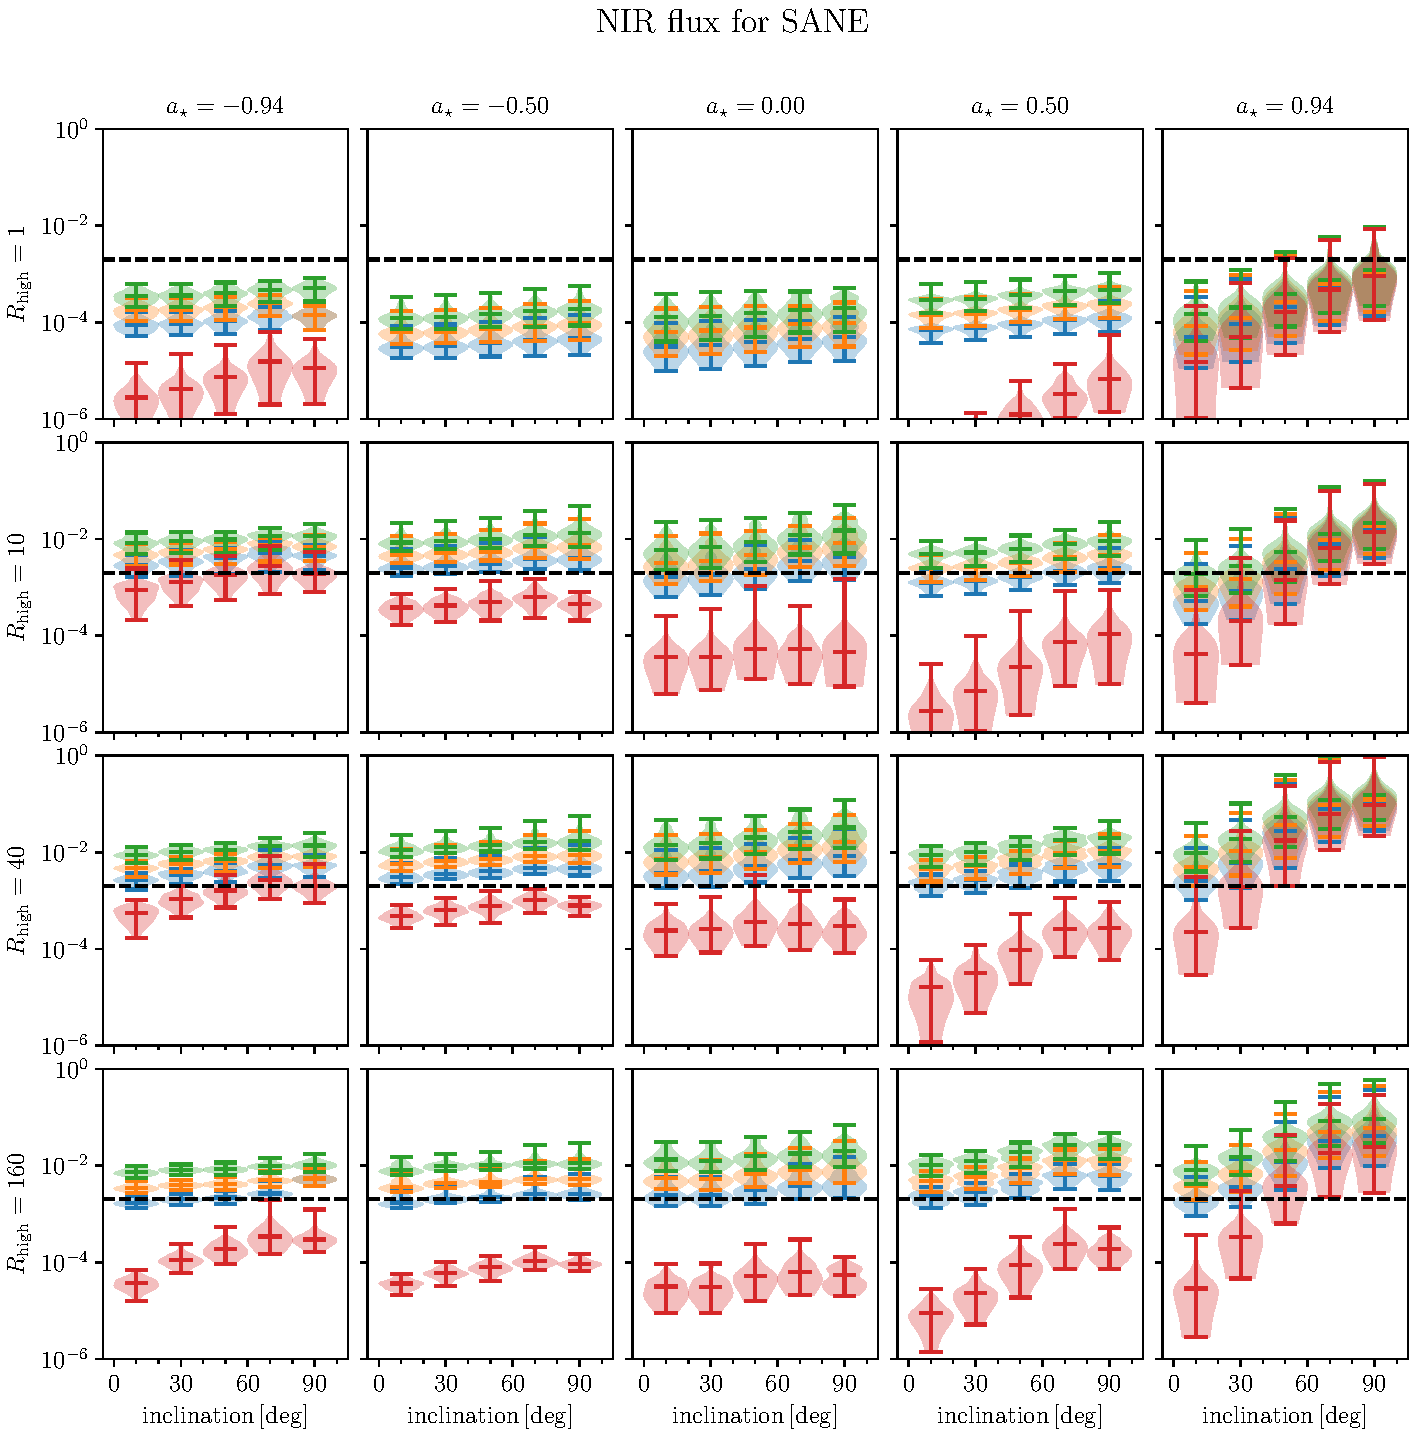
\includegraphics[width=\columnwidth]{./figures/SANE_NIR_standard.pdf}
  \caption{NIR constraints for SANE accretion models for thermal and non-thermal electron distribution function with $\kappa=3.4$ fixed and $\epsilon\left(\sigma,\beta,\varepsilon\right)$. The red violin plots correspond to a thermal eDF, blue, orange and green indicate kappa eDF with $\varepsilon=$0.05,0.1 and 0.2.}
  \label{fig:NIR_kappaepsilon}
\end{figure}

As can be seen in the figure, including non-thermal particles changes the distribution of the NIR fluxes significantly. Except for the $\Rh=1$ models the addition of non-thermal particles even with the lowest base efficiency used in this analysis $\left( \varepsilon=0.05\right)$ leads to a over-production of NIR fluxes. In the case of the MAD models all models over-produce the NIR flux for $\varepsilon=0.05$.

The NIR fluxes are produced by particles in the tail of the distribution function and are therefore are sensitive to slope of the tail. The emissivity for a thermal distribution decreases exponentially $\left(j_{\nu}\propto\exp(-\nu^{1/3})\right)$ while for the kappa distribution it behaves like $j_{\nu}\propto \nu^{-(\kappa-2)/2}$. Thus even at low base efficiencies, $\varepsilon$, the the flux from the kappa distribution in the NIR $\left(\nu\sim 10^{14}\,\rm{Hz}\right)$ is larger than for the thermal eDF.

%..............................................................................
\subsubsubsection{ALMA Light curves}

For the comparison with the ALMA light curves we compute the modulation index for a 3\,hour time window and across the entire simulated time window of 28\,hours (5000\,GM/c$^3$). Similar to the 86\,GHz flux the 230\,GHz flux is mainly produced within a few gravitational radii and thus not affected by the addition of non-thermal particles using Eq. \ref{eq:kappaeff}. As in the previous constraints, the MAD accretion models are insensitive to the addition of non-thermal particles whereas the SANE models show some increased modulation index for $\Rh>40$. However, the distributions for thermal and non-thermal eDF are still largely overlapping.

%..............................................................................
\subsubsubsection{m-ring}

The m-ring fitting is applied to the 230\,GHz images. As mentioned earlier the flux and size of the 230\,GHz images are not affected by the inclusion of non-thermal particles with fixed kappa and variable efficiency. Thus, we do not expect any changes in the distribution of the m-ring parameters.  Applying m-ring fitting to non-thermal models and a detailed comparison with the thermal results confirmed our initial assumption. \cmf{based on the results of Kotaro, who run the m-ring on non-thermal models}

%------------------------------------------------------------------------------
\subsubsection{Variable kappa model $\kappa(\sigma,\beta)$}

The non-thermal electron distribution function given in Equation \eqref{eq:nonthermaleDF} can be written in a general and self-consistent way by using a power-law slope dependent of the magnetisation $\sigma $ and plasma-$\beta$ from GRMHD simulations, $\kappa(\sigma, \beta)$, assuming that non-thermal particle acceleration due to magnetic reconnection following particle-in-cell small scale simulation from \citep{2018ApJ...862...80B}

\begin{align}
\kappa=2.8 +0.7\sigma^{-1/2} + 3.7\sigma^{-0.19}\tanh{(23.4\sigma^{0.26} \beta)}\label{eq:kappa} \\
w= \frac{ \kappa -3 }{\kappa} \Theta_{\rm e} + \frac{\varepsilon}{2}\left[1+\tanh(r-r_{\rm inj})\right]\, \frac{ \kappa -3 }{6 \kappa} \frac{m_{\rm p}}{m_{\rm e}} \sigma \label{eq:w}, 
\end{align}

where the width function contain thermal temperature and non-thermal contributions, second part defined by the magnetization and non-thermal particle acceleration efficiency \citep{2019A&A...632A...2D,2021NatAs.tmp..218C}. Although efficiency can be computed from first principles in PIC simulations
for convenience we only considered $\varepsilon=0$ and injection radius $r_{\rm inj}=10r_{g}$ following previous studies. Large heating efficiency $\varepsilon>0$ has large impact on NIR emission, the averaged flux increase two orders of magnitude when efficiency goes from 0 to 1, this implies that all passing models will overshoot NIR constraint, on the other hand, at 86GHz the flux increase around two times as well as the image size \citep{2021arXiv211102518F}. The emission, $j_{\nu}$, and absorption coefficients, $\alpha_{\nu}$, computed numerically can be found for the  interval $3< \kappa\leq 8$ in  \cite{2016ApJ...822...34P}. In order to compute the emission from regions where $\kappa$ is out of the validity range we use the thermal model, and neglect the emission in the jet spine, $\sigma > 1$ (see Figure \ref{fig:varepsilon}). 
\aco{Starting first draft}

%..............................................................................
\subsubsubsection{86\,GHz flux}

...
%..............................................................................
\subsubsubsection{86\,GHz image size}

...

\note{Razi, Angelo, Richard?}
\ckc{Write subsections only if they are different from the thermal models.}

%------------------------------------------------------------------------------
\subsubsection{Summary}

The effect of adding non-thermal particles via a kappa electron distribution function with fixed $\kappa=3.4$ values and variable efficiency via Eq.~\ref{eq:efficiencybetasigma} can be summarised in the following way:
\begin{itemize}
    \item The 86\,GHz and 230\,GHz constraints are hardly effected by the addition of non-thermal particles.
    \item Even the lowest a base efficiency considered, $\varepsilon=0.05$, leads to an over-production of NIR flux. \cmf{indication that we need very localised regions of non-thermal particle productions and no "global" approach?}
\end{itemize}

\note{Alejandro to write here about Frankfurt nonthermal models.  Define a subsection, describe the results and how they differ from the thermal results.}

\note{Tomohisa to write here about UWABAMI nonthermal power-law models}

\ckc{Write subsections only if they are different from the thermal models.}

%==============================================================================
\subsection{Tilted Models}

\note{Koushik to write here.  Describe the results and how they differ from aligned thermal results.}
\ckc{Write subsections only if they are different from the thermal models.}

%==============================================================================
\subsection{Stellar Wind Fed Models}

\note{Angelo and George to write here.  Describe the results and how they differ from aligned thermal results.}
\ckc{Write subsections only if they are different from the thermal models.}

%==============================================================================
\subsection{Best Bet Models}

\begin{figure*}
    \centering
    \note{altex: a grid figure showing the $\sim$ 4 best bet models.  Each model in a column.  Top two rows are the 230GHz images and 86GHz images, last row is SEDs.}
    \caption{Best bet models.  Each column corresponds to one best bet model; top row shows a 230GHz image \note{average or selected image; or use GIF?}; middle row shows an 86GHz images; bottom row shows SEDs.}
    \label{fig:my_label}
\end{figure*}

\note{Michi to provide first draft}

We now consider combined constraints, excluding variability, under the hypothesis that (1) there is a missing physical ingredient in the models that would lower variability, but (2) that missing ingredient would not vitiate the models entirely.  Models are eliminated if they fail any one constraint.

Figure showing combined constraints for thermal models.

Figure showing combined constraints for nonthermal models.

We then inspected the remaining models and selected four best-bet models that approximately span the space of successful models.  \note{Written characterization of remaining models; possibly 3 or 5}
